\chapter{Bewertung der zusätzlichen Klauseln}
\label{chp:bewertung}

Die erhaltenen Klauseln aus Kapitel \ref{chp:analyse} werden in diesem Abschnitt darauf überprüft,
ob und wie sehr sie den Lösungsprozess beschleunigen oder ausbremsen. Die Berechnungen wird auf einem
Server mit folgenden Eigenschaften durchgeführt:
\begin{itemize}
  \item Fedora 22
  \item 2 x Intel(R) Xeon(R) CPU E3-1240 V2 (3.40GHz)
  \item 2 x 4 Kerne (8 Threads)
  \item 32Gb RAM
  \item 16Gb Auslagerungsdatei
\end{itemize}

Wie auch für die Ermittlung der Klauseln in Kapitel \ref{chp:analyse} wird eine Urbildberechnung (siehe Abschnitt \ref{sec:urbildberechnung})
für die Bewertung herangezogen. Eine annähernd sinnvolle Zeitmessung ist erst möglich, wenn mindestens neun Bits des \glos{hash}{s} vorgegeben werden.
Die obere Grenze liegt bei 22 Bits, bei denen die genutzte Hardware noch zuverlässig zu einer Lösung kommt. Da CryptoMiniSat in der Standardkonfiguration
mit acht Threads während des Lösungsprozesses Werte rät, kann es zufällig zu schnellen Lösungen kommen. Um ein aussagekräftiges Ergebnis
zu bekommen, werden für neun bis 22 Bit jeweils fünf Versuche durchgeführt. Betrachtet wird auch jeweils eine Version mit und ohne XOR-Klauseln.

Um die Ergebnisse kompakt darstellen zu können, werden diese in Diagrammen dargestellt die mit der Legende in Abbildung \ref{fig:data_lengede}
kurz erläutert werden sollen. Jede Spalte in der X-Achse stellt 5 Versuche dar, die mit der jeweils festgelegten Anzahl der Bits im \glos{hash}
durchgeführt wurden. Die linke Y-Achse repräsentiert die Dauer in Sekunden. Da die Dauert im Bezug zu der Anzahl der vorgegebenen Bits exponentiell
wächst, ist die Y-Achse logarithmisch skaliert. Die grünen Balken zeigen, in welchem Bereich die Ergebnisse der fünf Versuche liegen, wobei
der blaue Punkt das arithmetische Mittel darstellt. Die rechte Y-Achse stellt die Anzahl der unterschiedlichen Ergebnisse dar, die durch die
roten Punkte markiert werden. Dieser gibt somit einen Hinweis, wie viel Raten und somit Zufall bei der Lösung im Spiel war. Kommt CryptoMiniSat
bei allen fünf Versuchen zum selben Ergebnis, haben die Heuristiken gut funktioniert und es musste wenig geraten werden. Das spiegelt sich auch
darin wieder, dass die Dauer der fünf Versuche sich wenig unterscheidet.
\begin{figure}[!h]
  \centering
  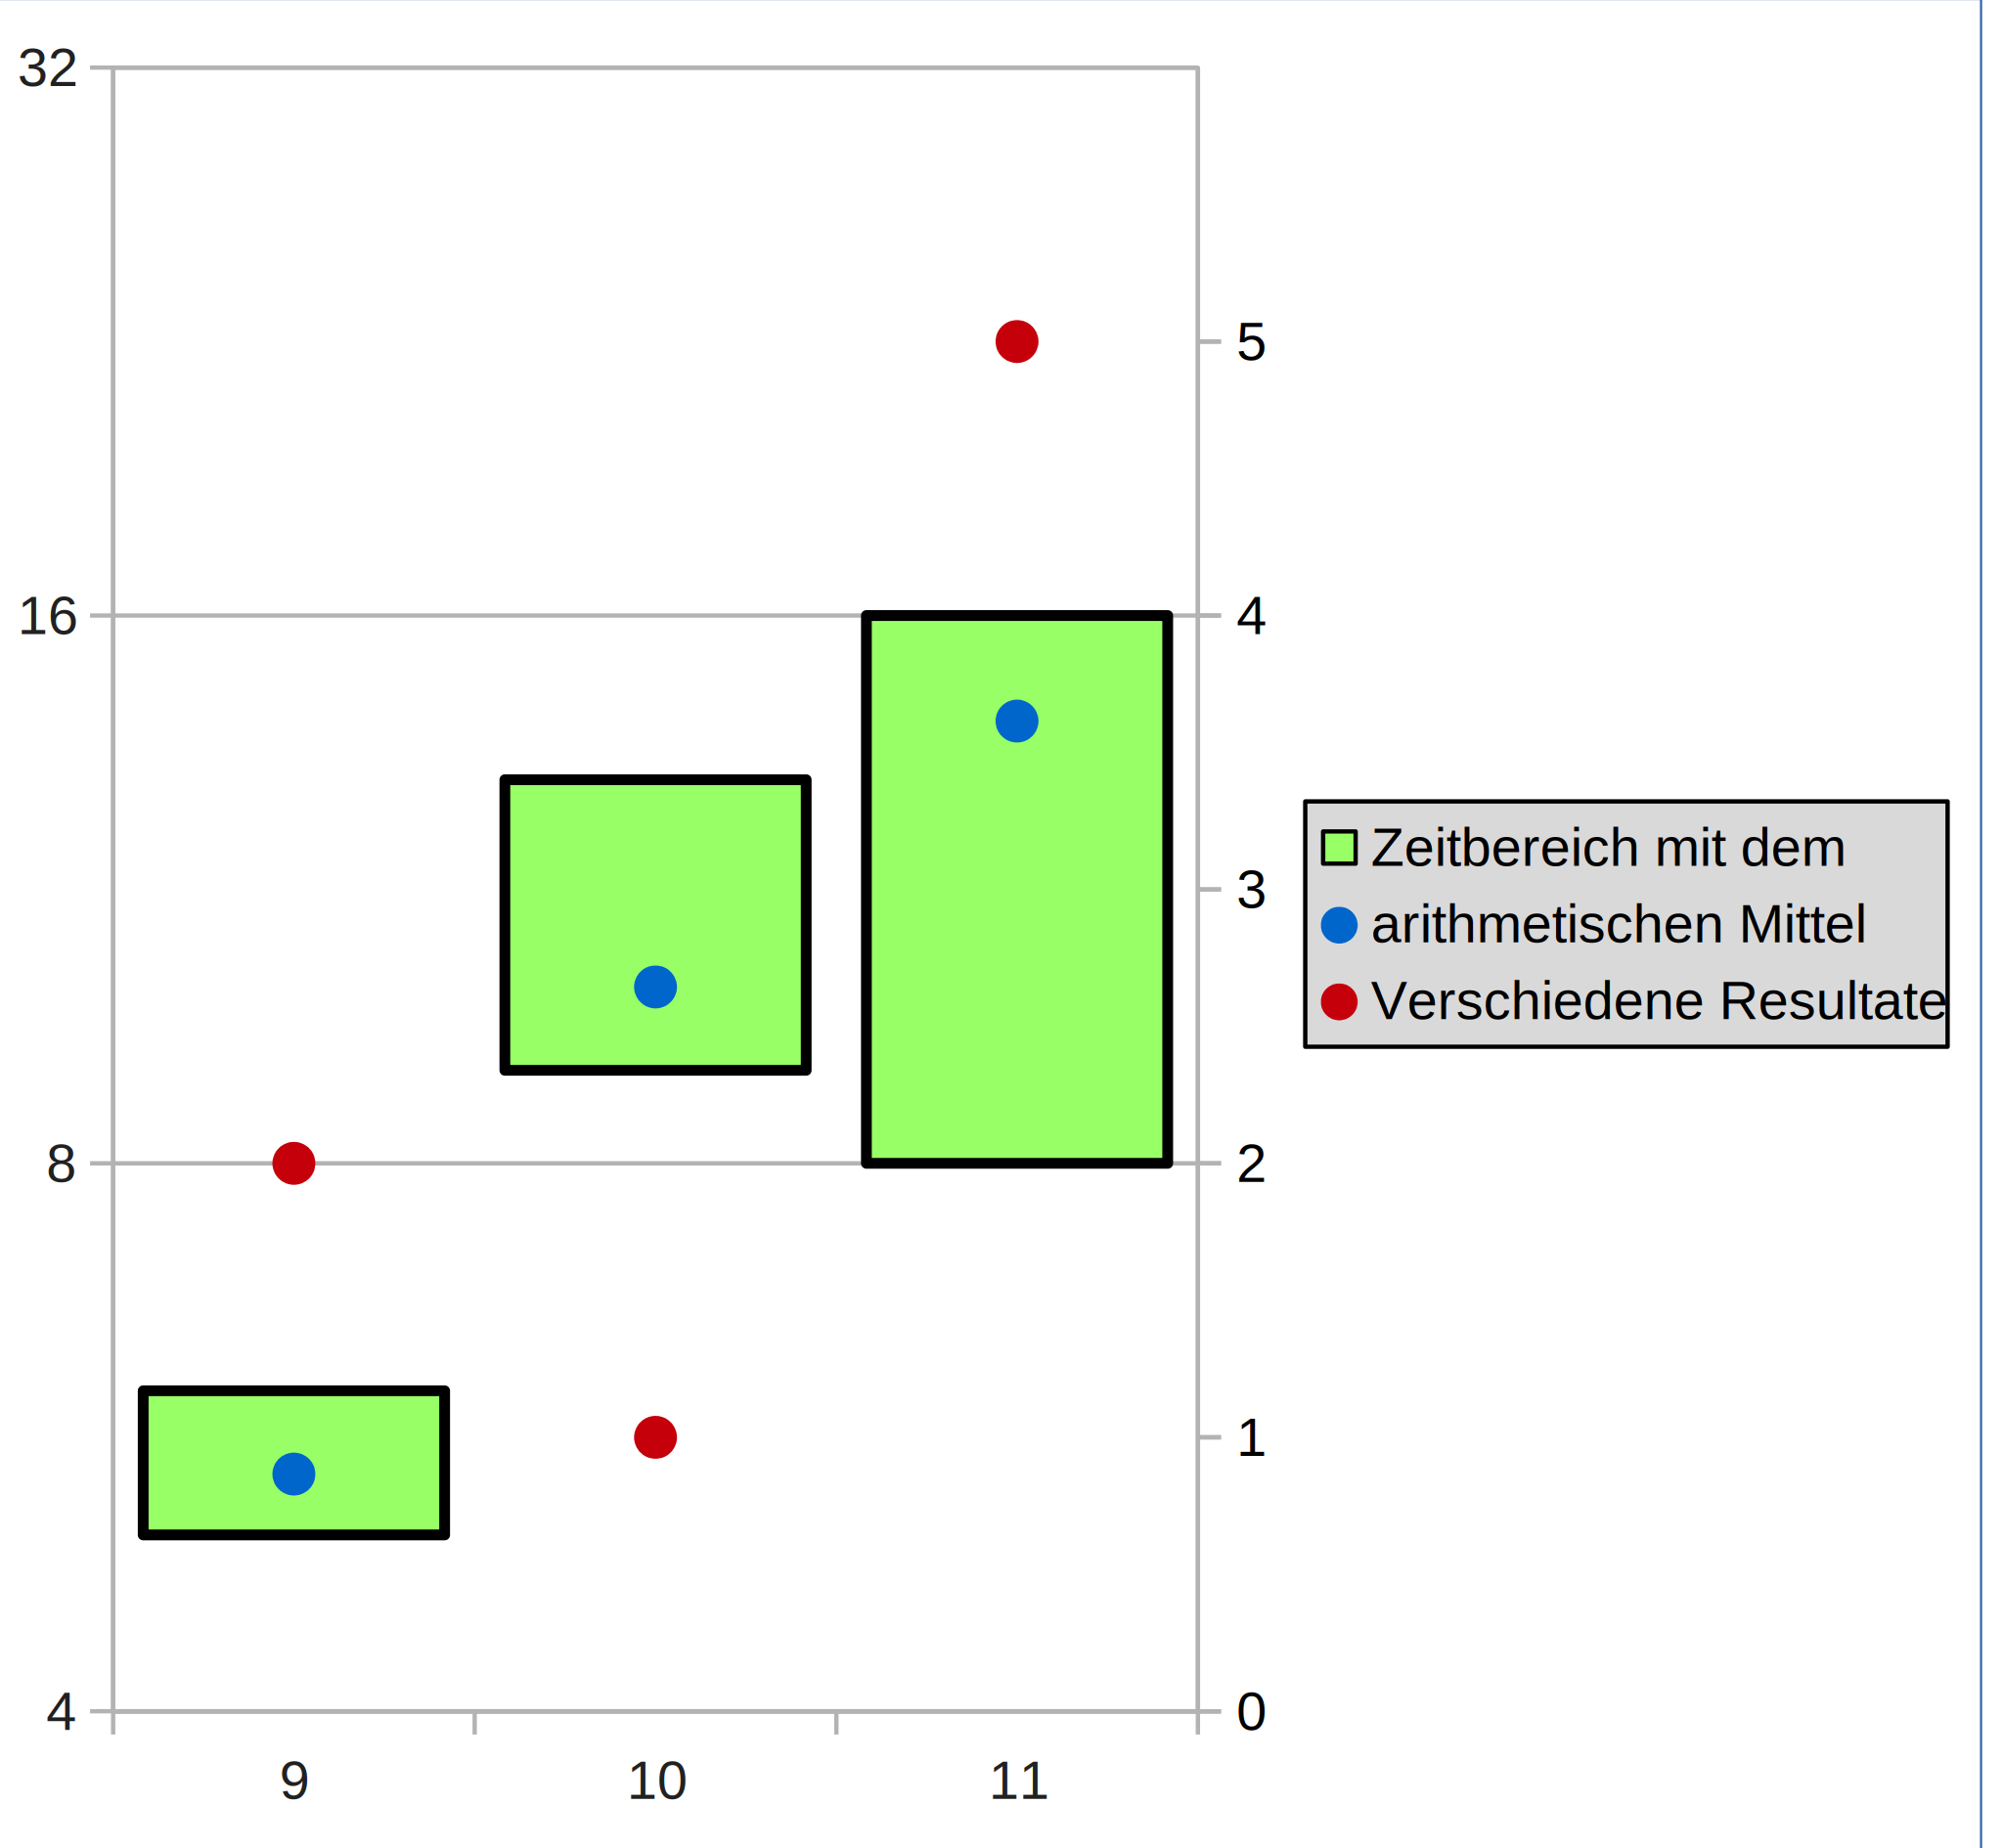
\includegraphics[scale=0.55]{images/data_legend}
  \caption{Legende}
  \label{fig:data_lengede}
\end{figure}

Als Vergleichsbasis dient die konjunktive Normalform aus Kapitel \ref{chp:knf} ohne zusätzliche Klauseln. Die Ergebnisse sind in
Abbildung \ref{fig:data_base} dargestellt. Es zeigt sich, dass die XOR-Variante insgesamt ein wenig schneller ist. Auffällig ist,
dass die Zeit für die Variante ohne XOR sich im Bereich von 11 bis 15 Bit nur verdoppelt und bei 16 Bit ein Sprung erfolgt. In
diesem Bereich hat die XOR-Variante einen Nachteil. Bezüglich der Anzahl der unterschiedlichen Ergebnisse gibt es keine relevanten
Unterschiede.
\begin{figure}[!h]
  \centering
  \begin{minipage}[t]{0.45\textwidth}
  \begin{flushleft}Gesamtdauer ohne XOR: 194:27:41\end{flushleft}
  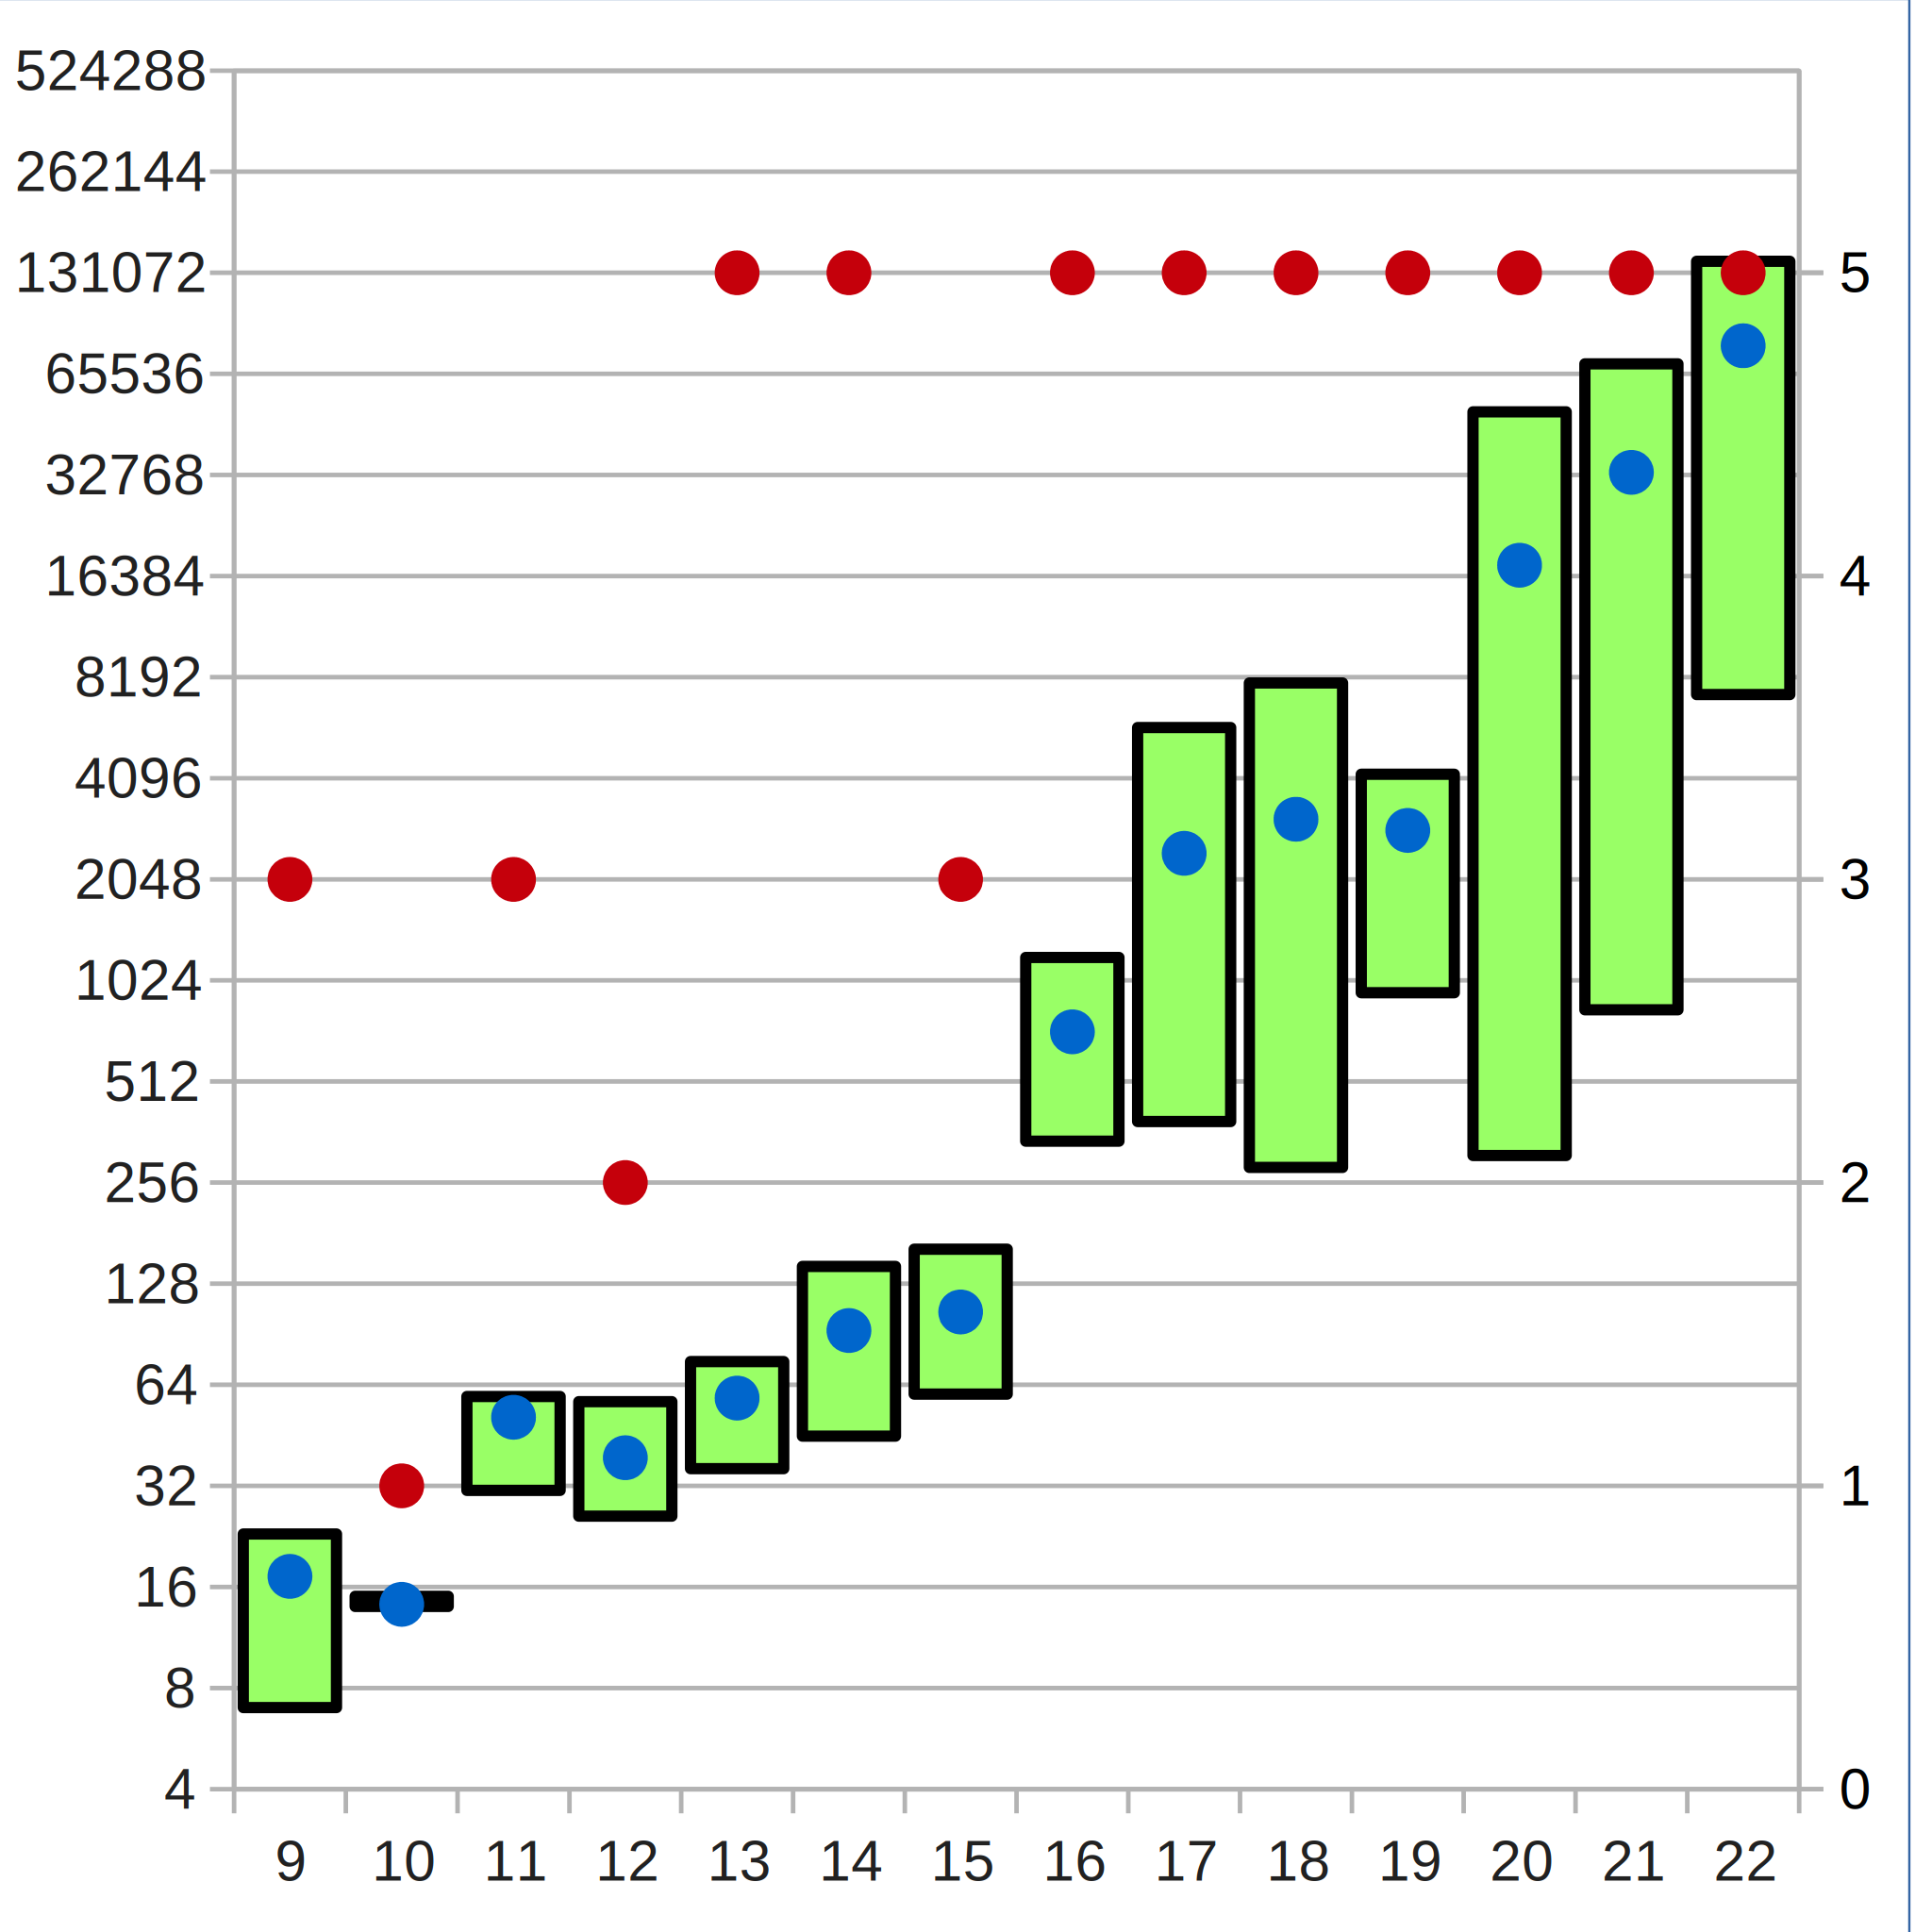
\includegraphics[scale=0.55]{images/data_base_knf}
  \end{minipage}
  \begin{minipage}[t]{0.09\textwidth}
  ~~
  \end{minipage}
  \begin{minipage}[t]{0.45\textwidth}
  \begin{flushleft}Gesamtdauer mit XOR: 169:24:12\end{flushleft}
  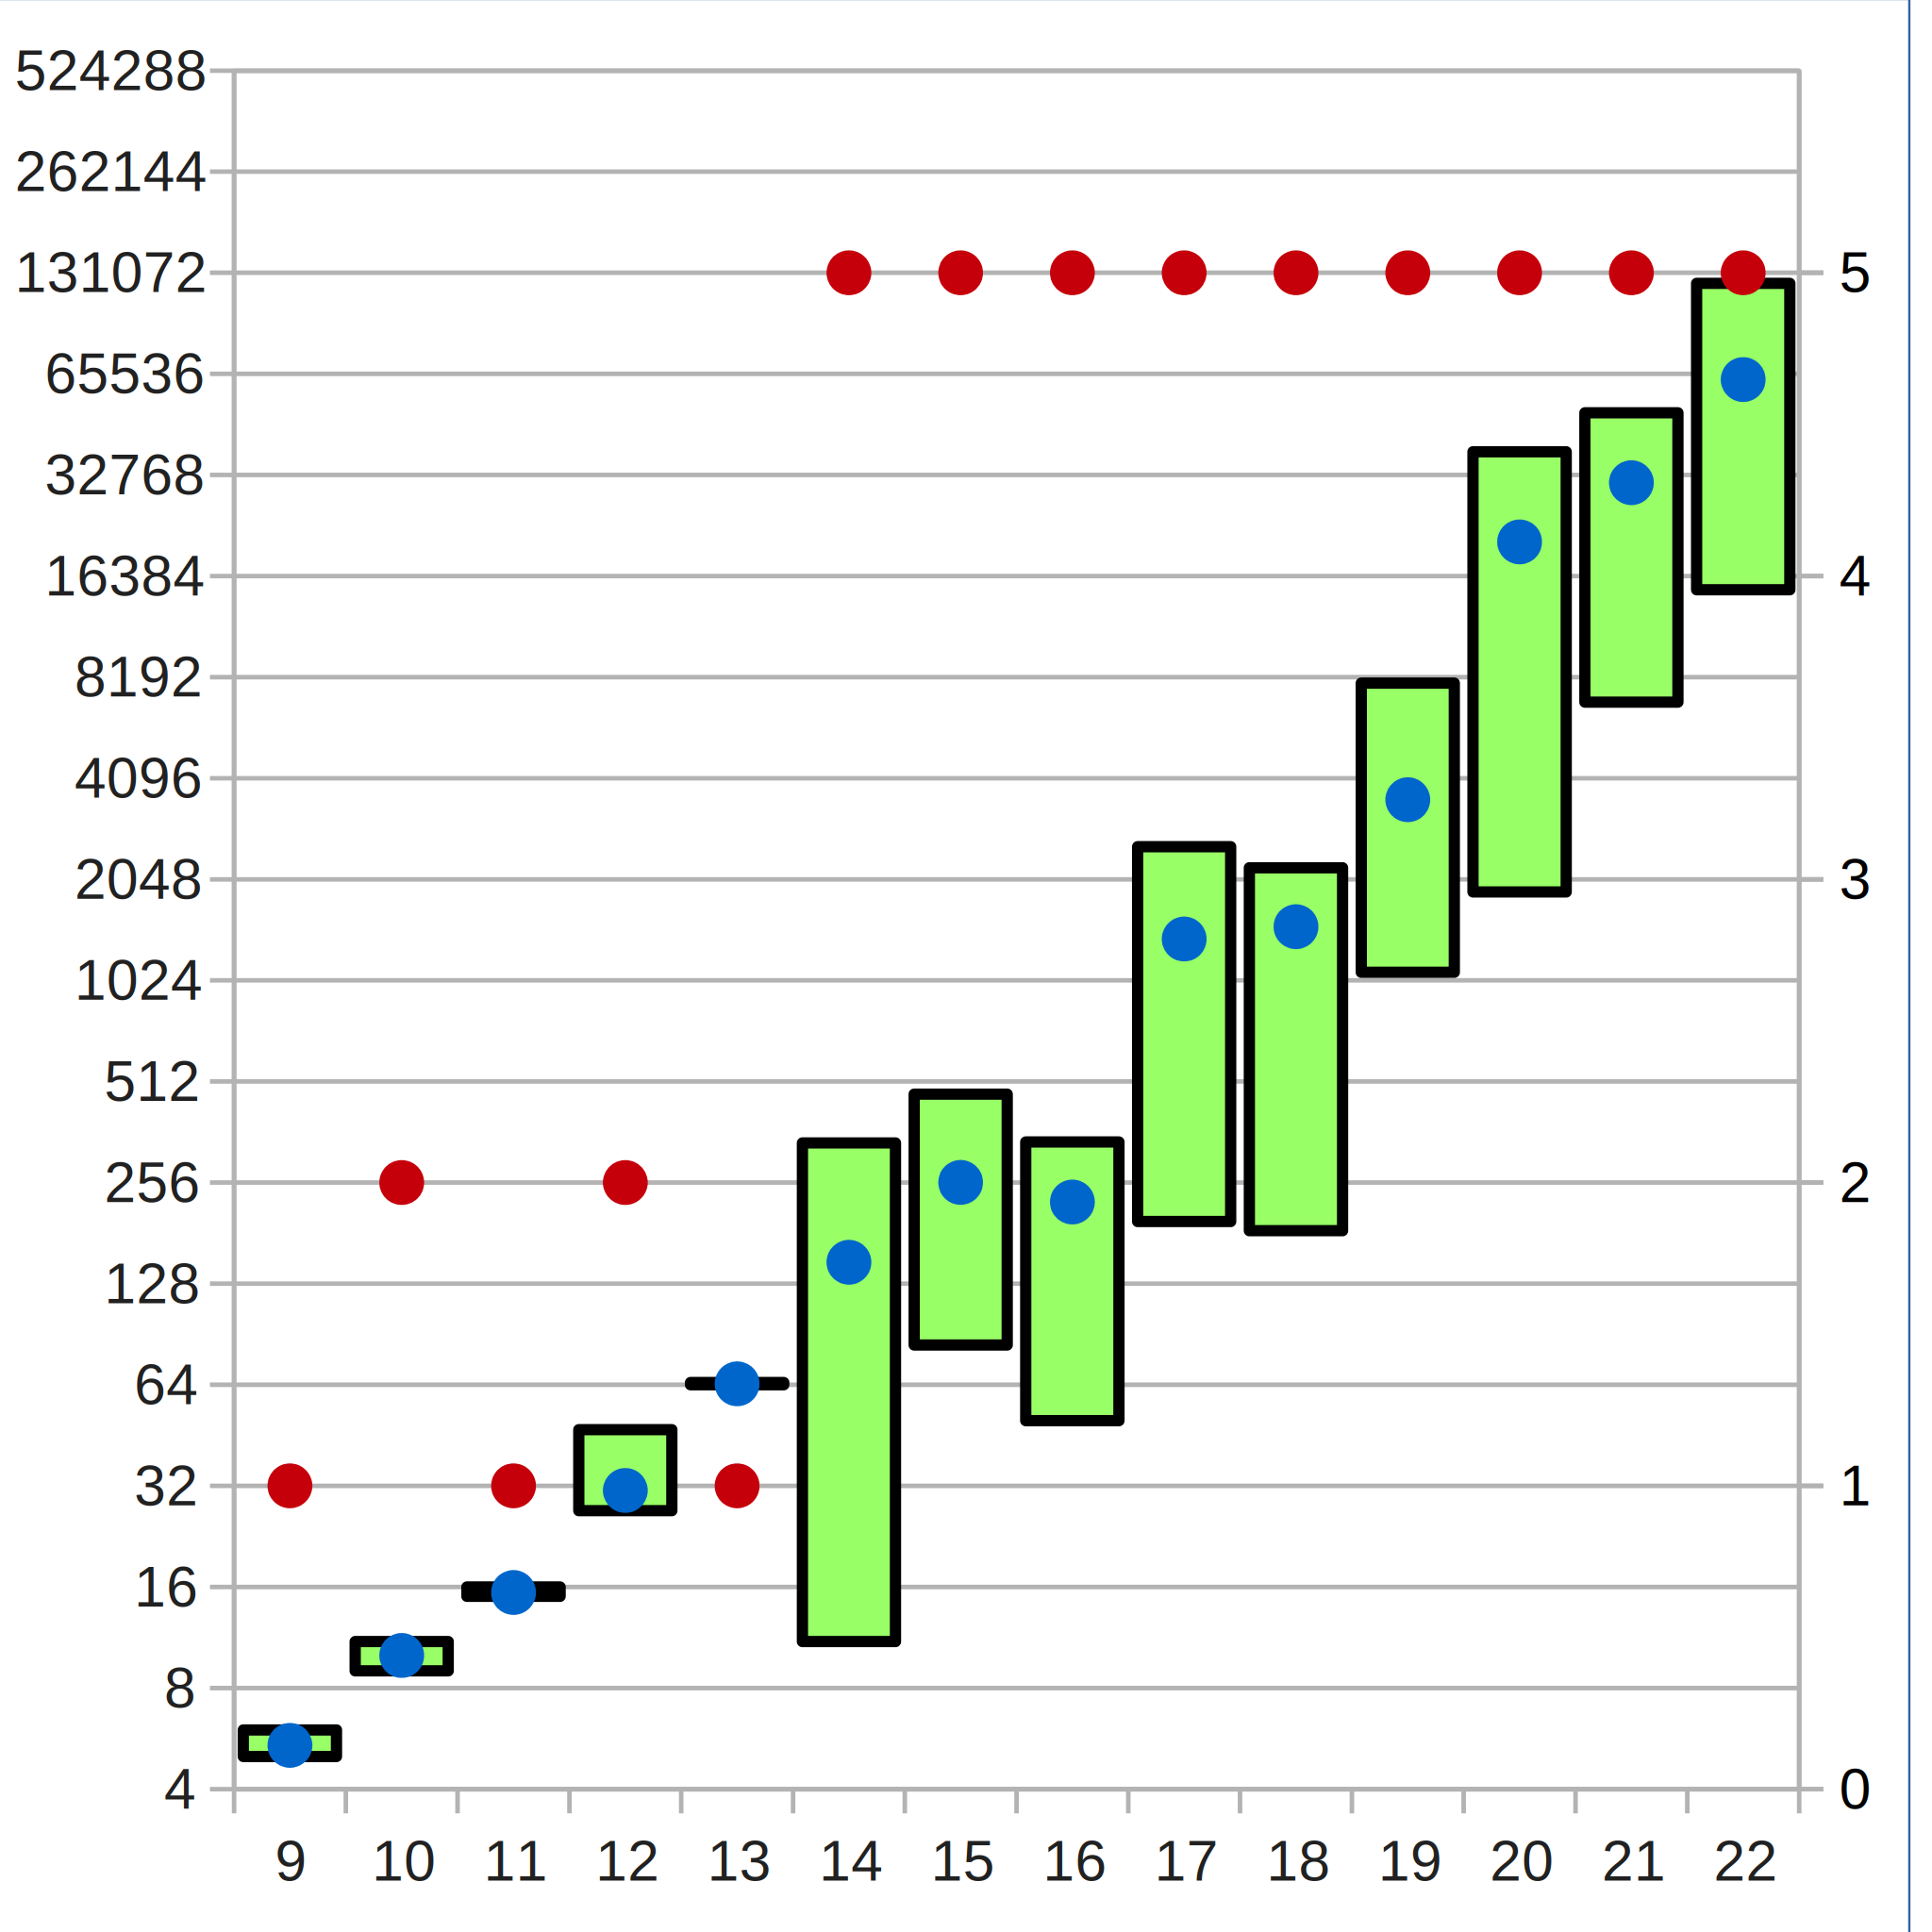
\includegraphics[scale=0.55]{images/data_base_xor}
  \end{minipage}
  \caption{Vergleichsbasis}
  \label{fig:data_base}
\end{figure}

\section{Test mit modulspezifischen Klauseln} % 47 - 41
\label{sec:test_modul}

Dieser Test bezieht zusätzlich zu den Basisklauseln die Klauseln aus Tabelle \ref{fig:additional_clauses_mod} mit ein.
Ausgenommen sind davon jedoch die zusätzlichen Klauseln für den Addierer, die in Abschnitt \ref{sec:test_234} separat getestet werden.
Die Ergebnisse sind in Abbildung \ref{fig:data_modul} dargestellt.
Insgesamt reduziert sich die Testlaufzeit um mehr als 50\% wobei die XOR-Variante nach wie vor schneller ist.
Ein weiterer Vorteil der XOR-Variante in diesem Test ist die Anzahl der unterschiedlichen Ergebnisse. Durch die
zusätzlichen Klauseln konnte CryptoMiniSat mehr Berechnungen durchführen und das Raten von Belegungen vermeiden.
\begin{figure}[!h]
  \centering
  \begin{minipage}[c]{0.45\textwidth}
  \begin{flushleft}Gesamtdauer ohne XOR: 91:28:43\end{flushleft}
  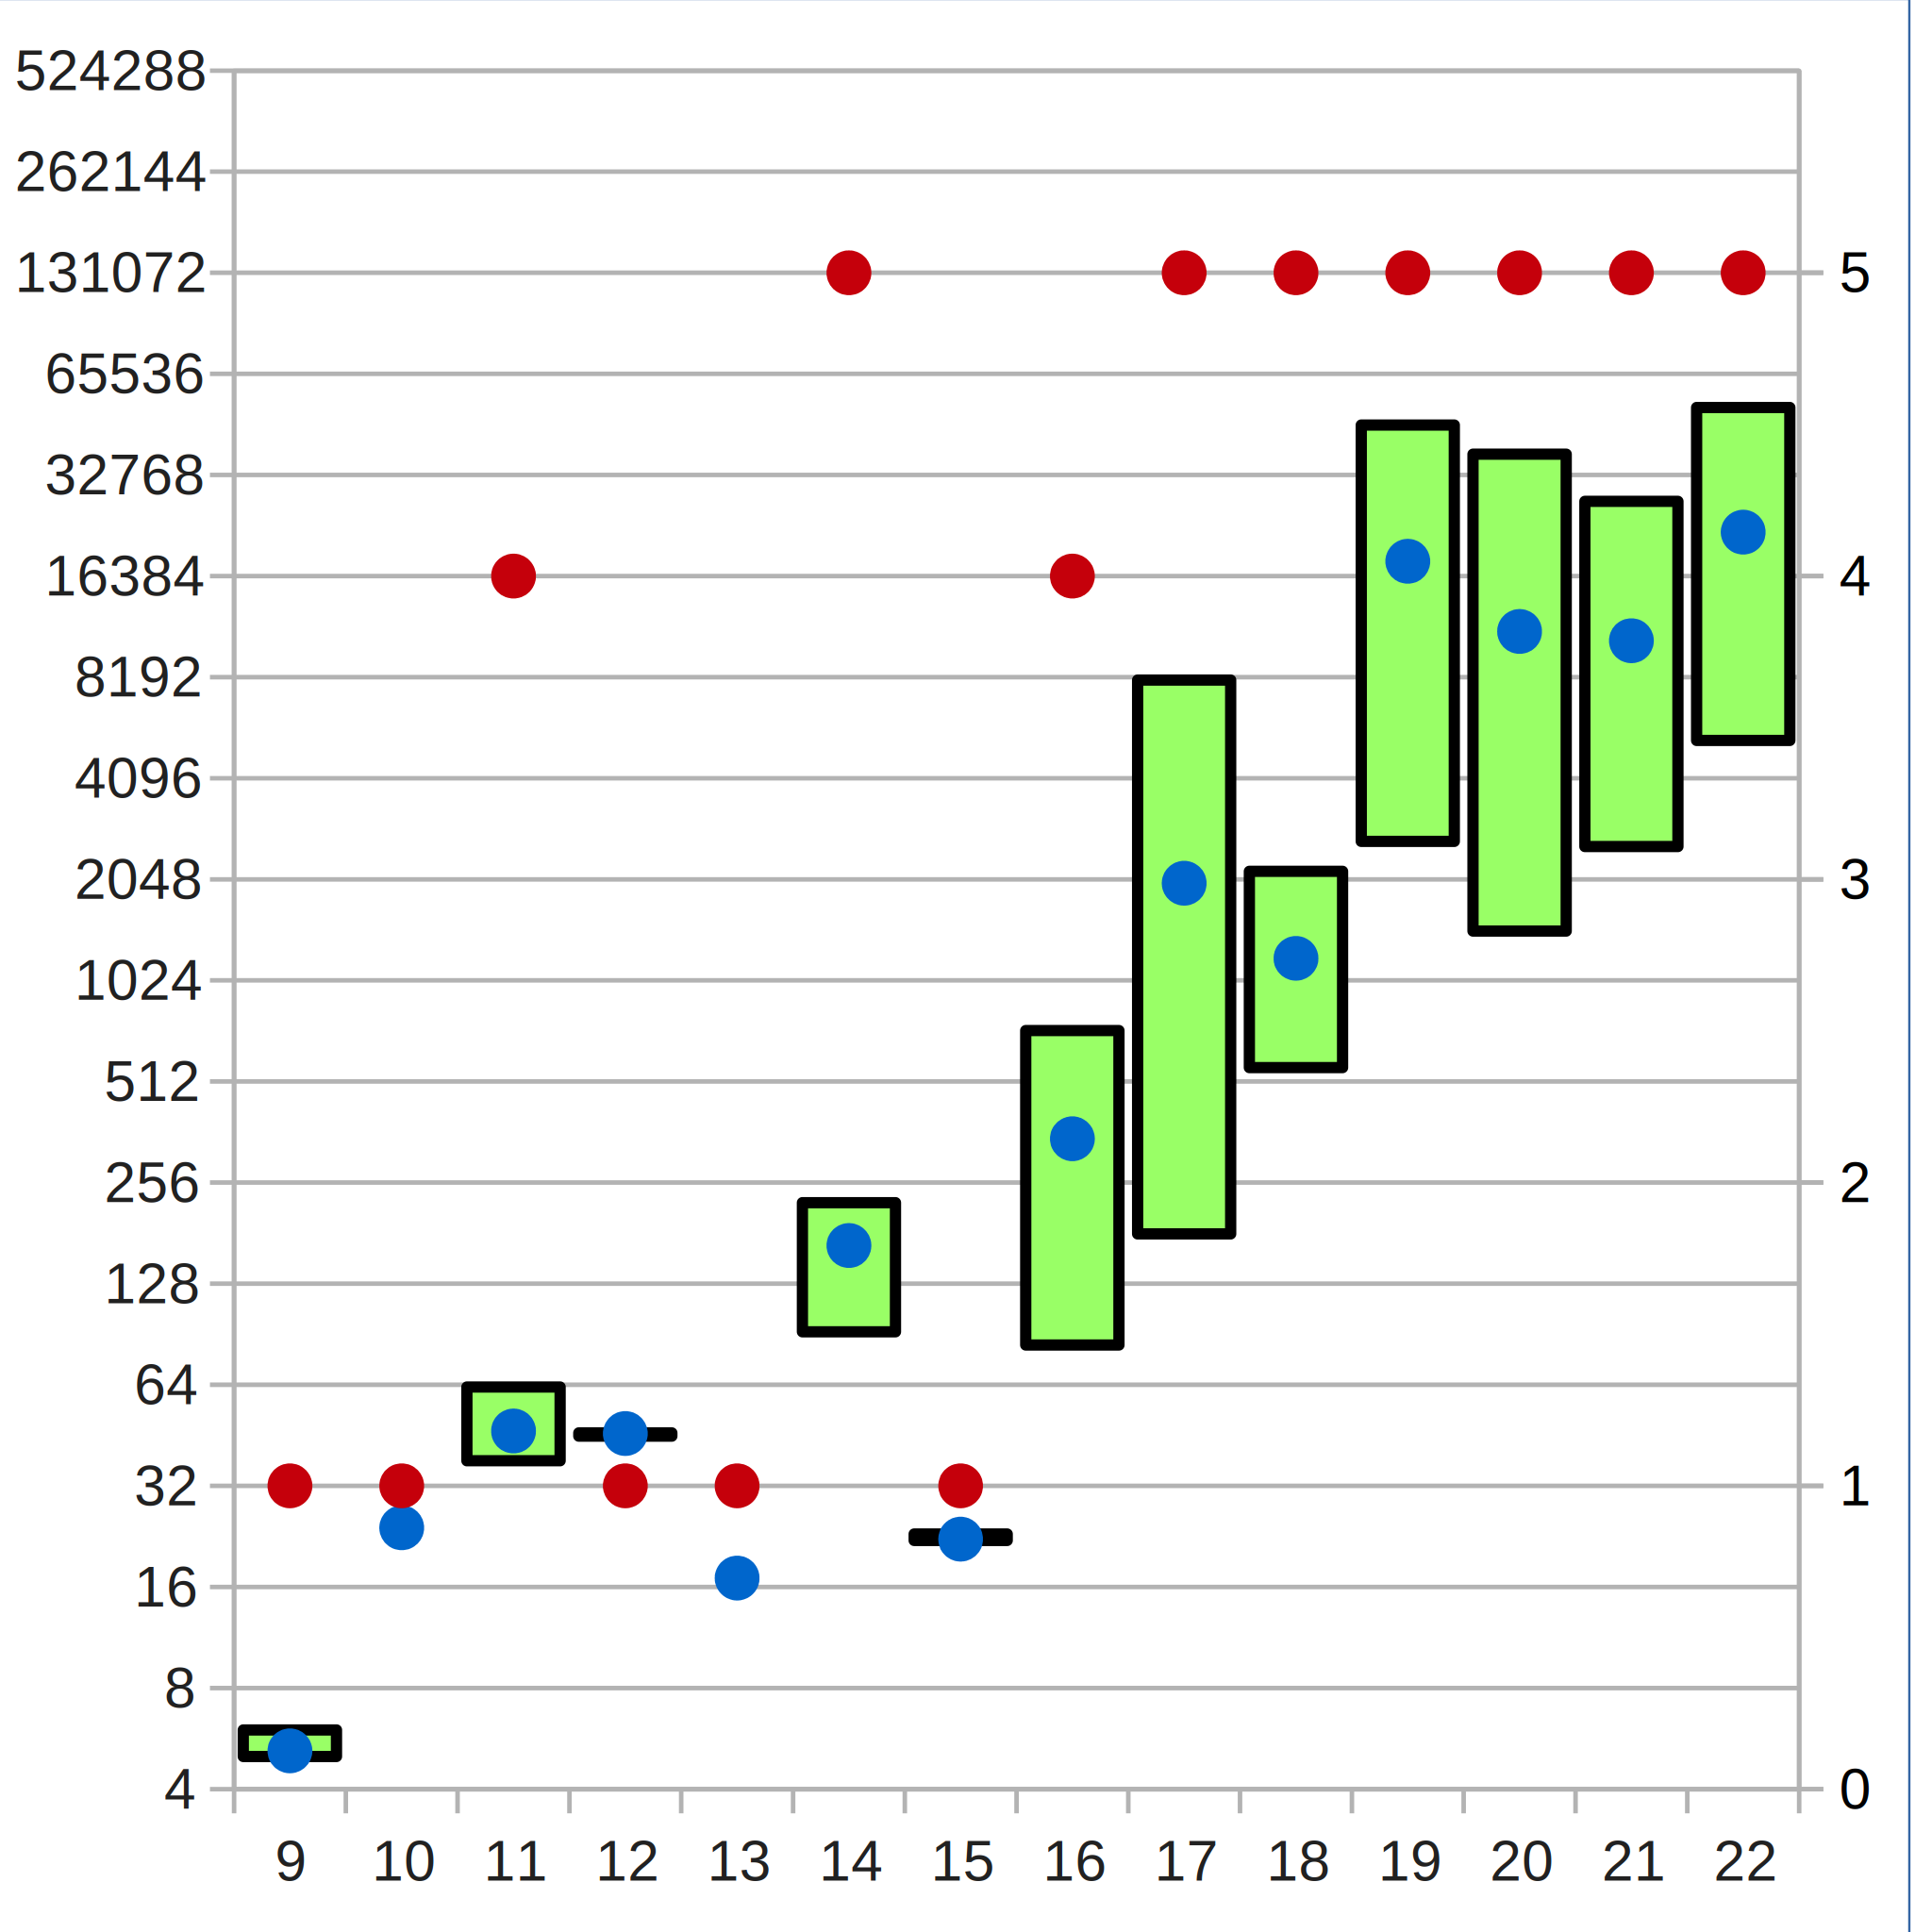
\includegraphics[scale=0.55]{images/data_modul_knf}
  \end{minipage}
  \begin{minipage}[c]{0.09\textwidth}
  ~~
  \end{minipage}
  \begin{minipage}[c]{0.45\textwidth}
  \begin{flushleft}Gesamtdauer mit XOR: 69:07:57\end{flushleft}
  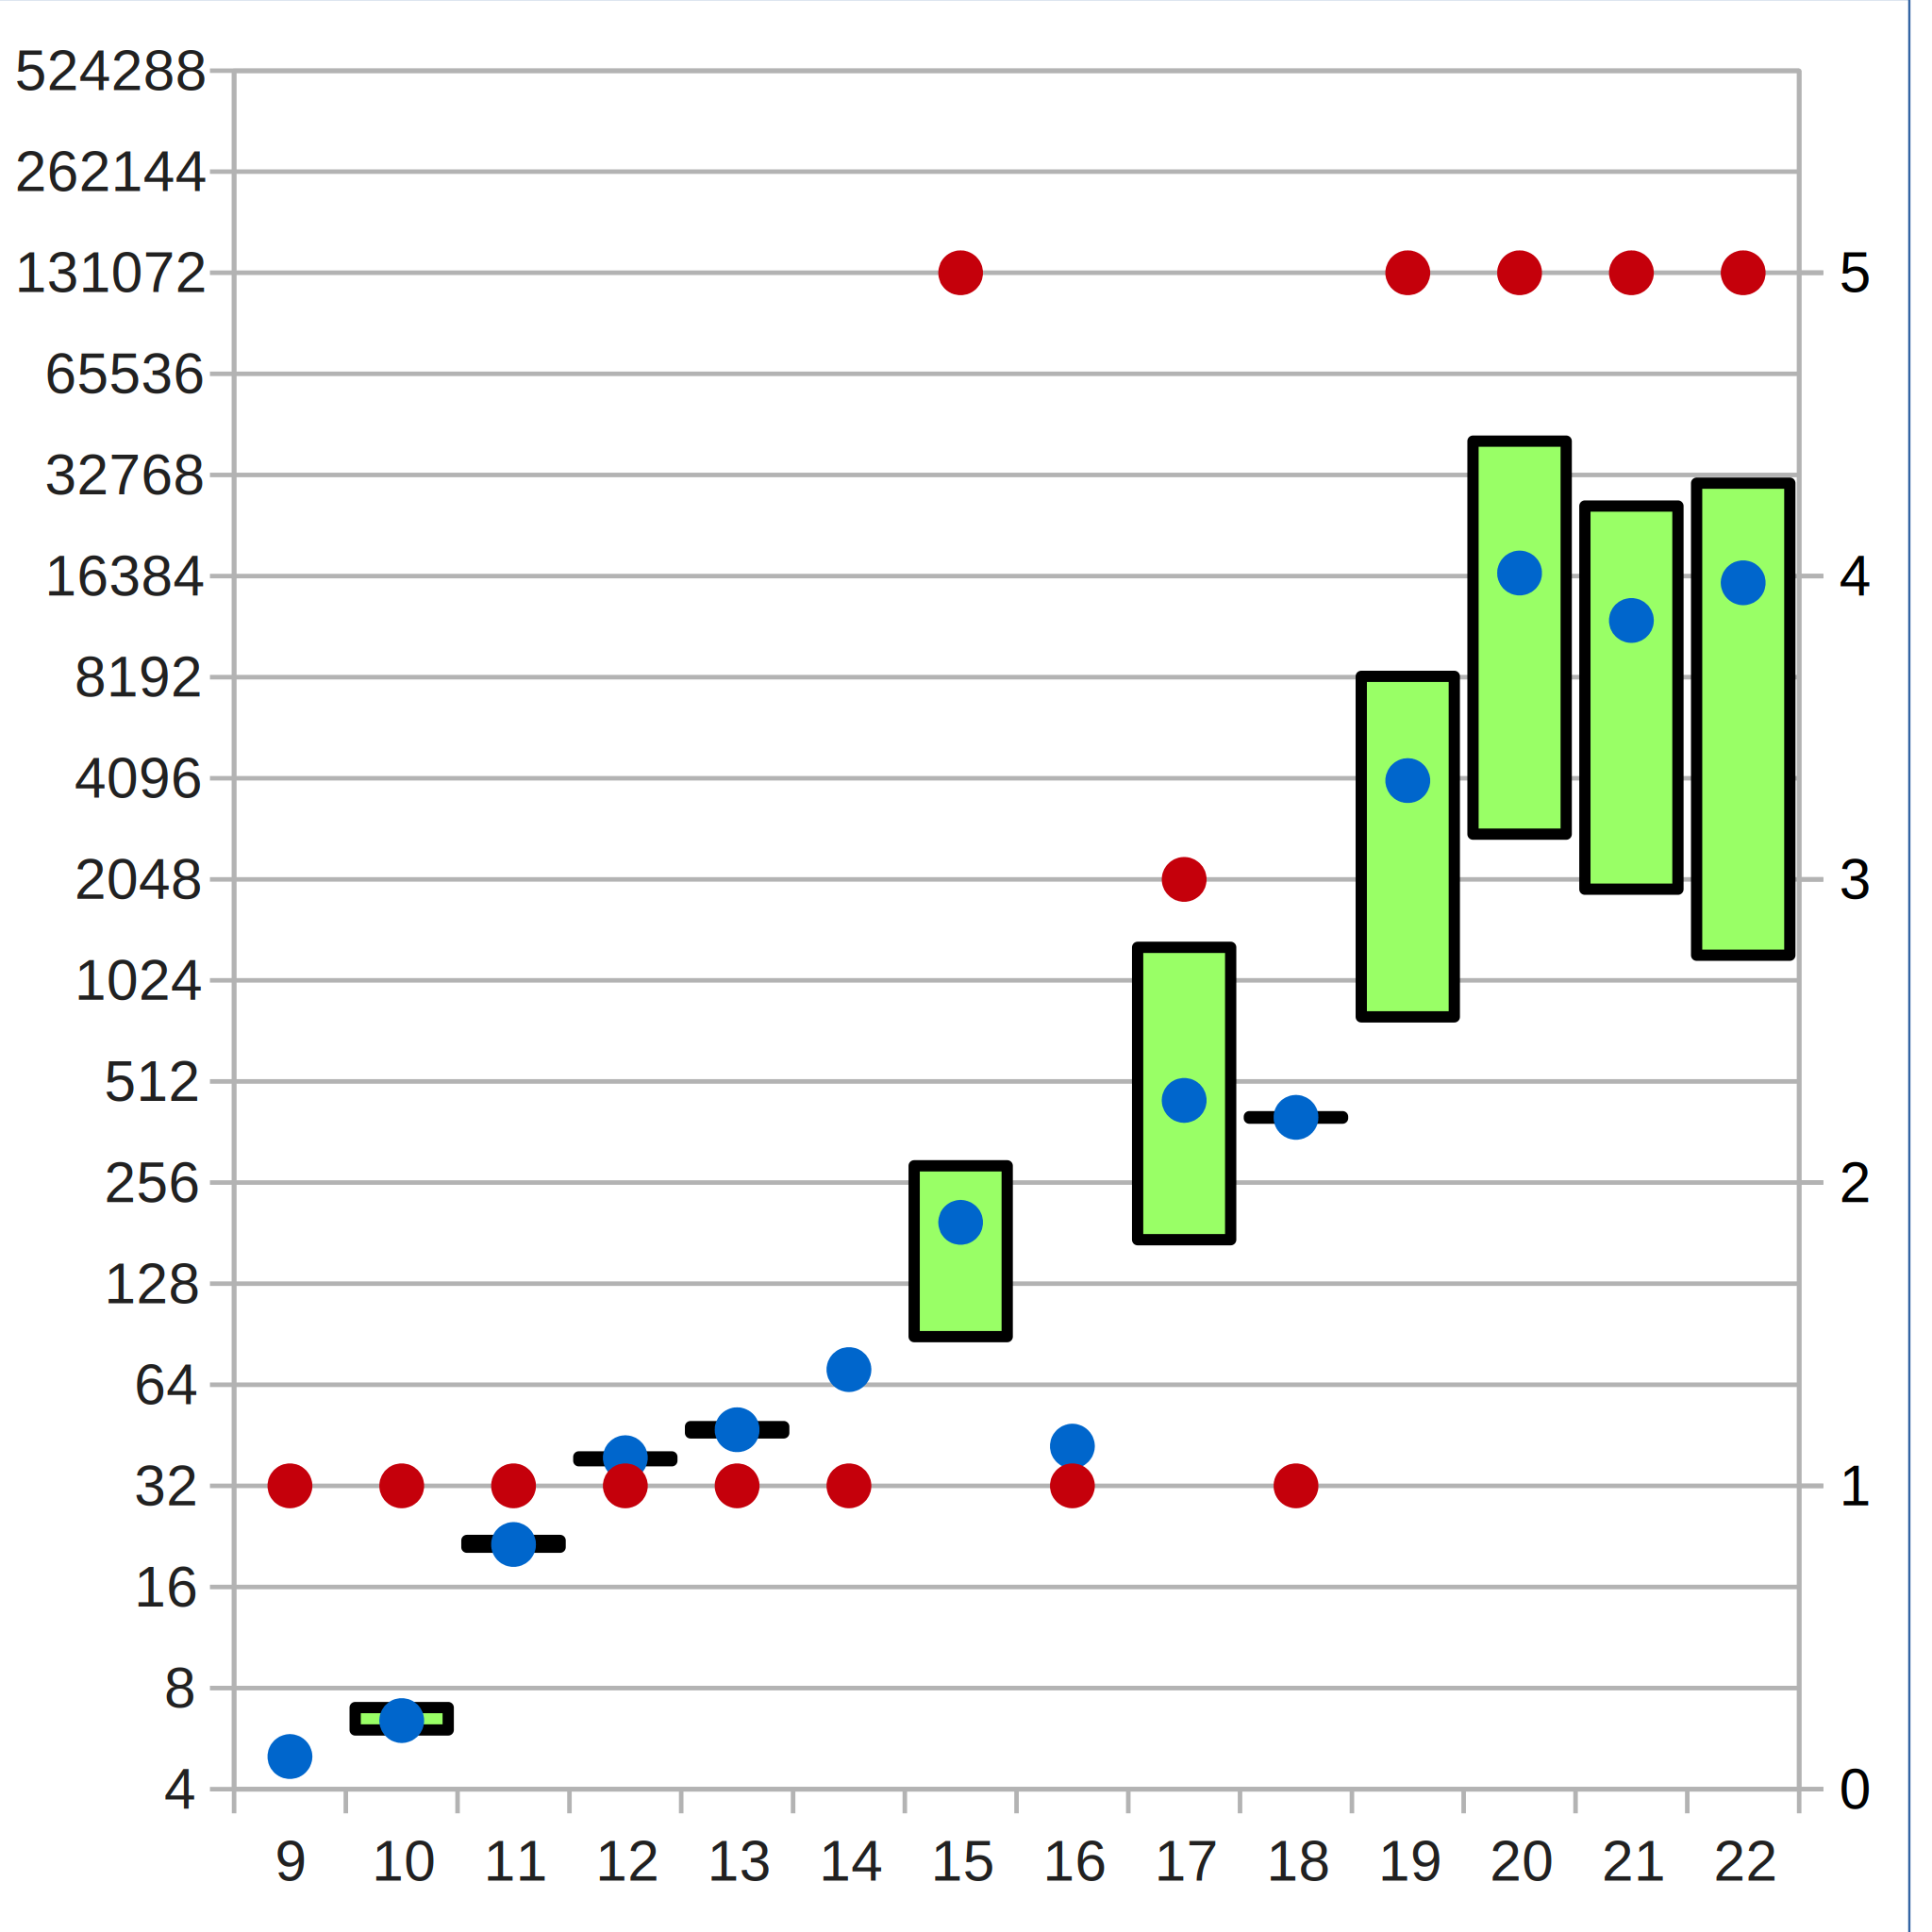
\includegraphics[scale=0.55]{images/data_modul_xor}
  \end{minipage}
  \caption{Ergebnisse mit modulspezifischen Klauseln}
  \label{fig:data_modul}
\end{figure}
\section{Test mit Distanzklauseln} % 80 - 83
\label{sec:test_distanz}

In diesem Test werden zusätzlich zu den Basisklauseln die Klauseln aus Tabelle  \ref{fig:additional_clauses_clean} mit einbezogen.
Die Ergebnisse sind in Abbildung \ref{fig:data_dist} dargestellt.
Auch hier reduziert sich die Testlaufzeit. Im Vergleich zu den modulspezifischen Klauseln reduziert sich die Laufzeit nur um 20\%
anstatt 50\%. Genau entgegen gesetzt ist jedoch das Verhalten bezüglich der Anzahl der unterschiedlichen Lösungen. Diese Klauseln
führen dazu, dass mehr geraten und weniger berechnet wird. Wie auch bei den Basisklauseln lässt sich in der Variante ohne XOR-Klauseln
ein Sprung der Lautzeit nach oben erkennen. Dieser erfolgt bei diesem Test jedoch erst bei 17 Bit.
\begin{figure}[!h]
  \centering
  \begin{minipage}[c]{0.45\textwidth}
  \begin{flushleft}Gesamtdauer ohne XOR: 155:31:37\end{flushleft}
  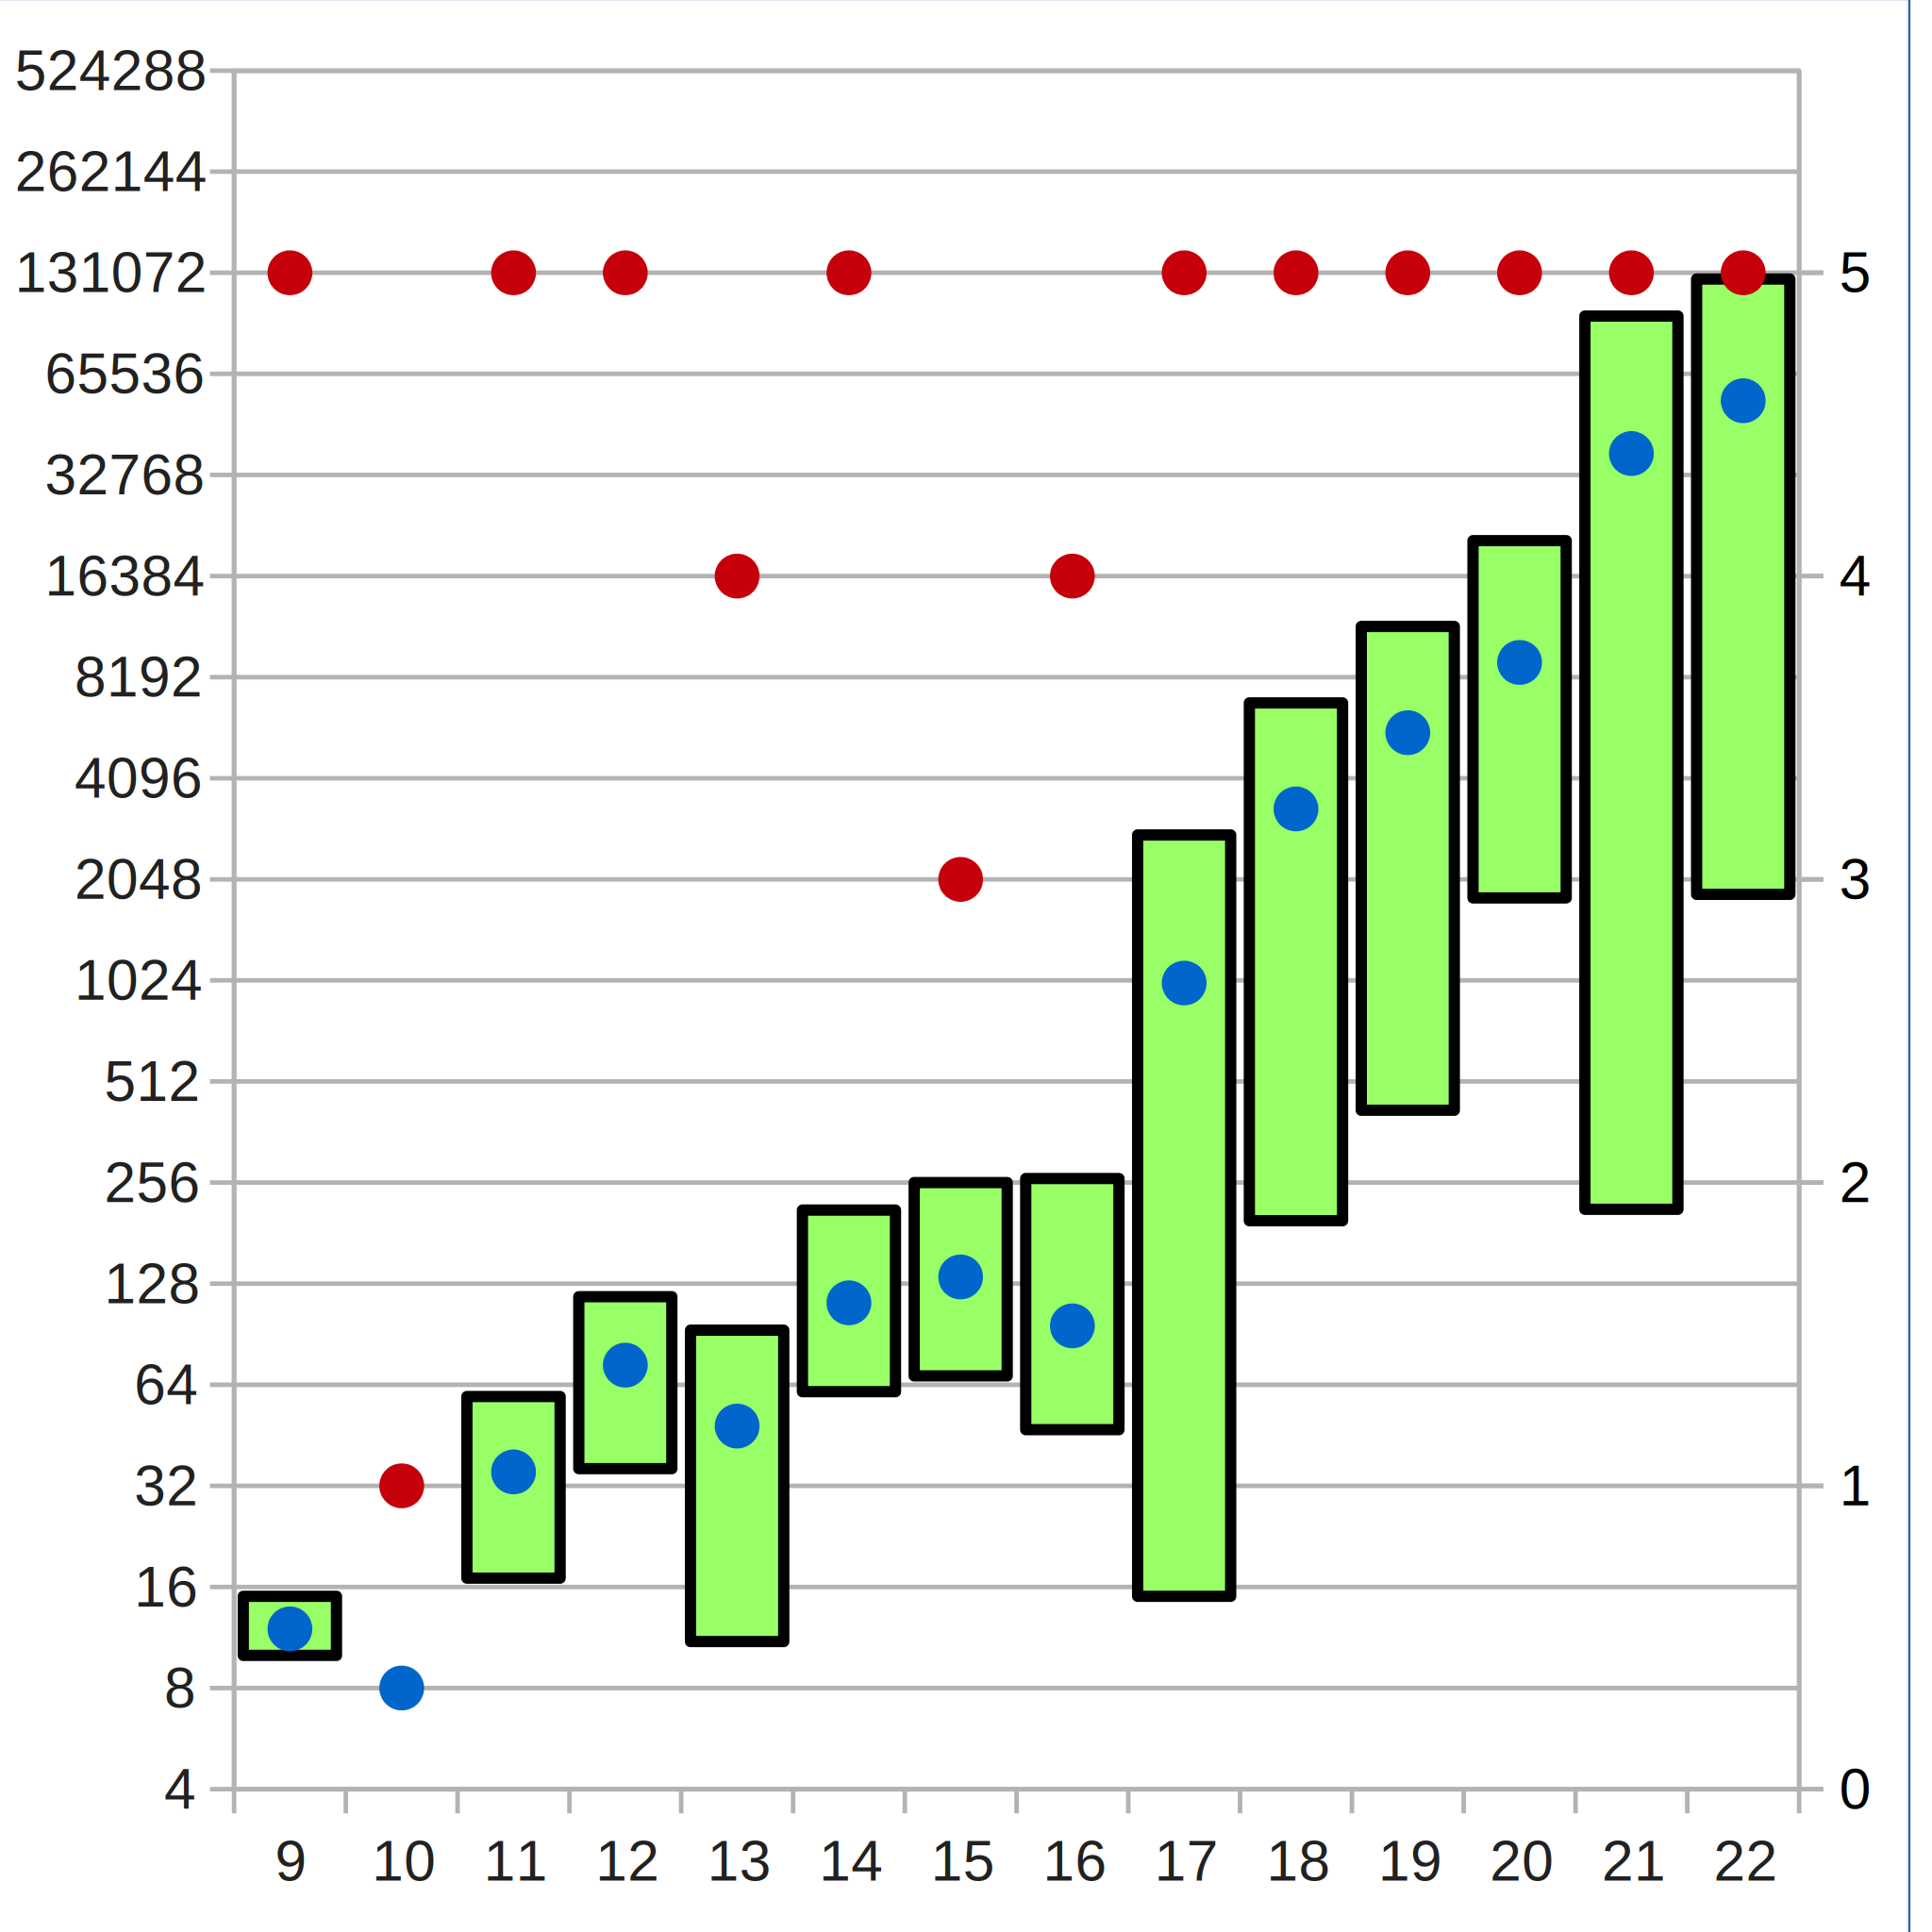
\includegraphics[scale=0.55]{images/data_dist_knf}
  \end{minipage}
  \begin{minipage}[c]{0.09\textwidth}
  ~~
  \end{minipage}
  \begin{minipage}[c]{0.45\textwidth}
  \begin{flushleft}Gesamtdauer mit XOR: 141:34:35\end{flushleft}
  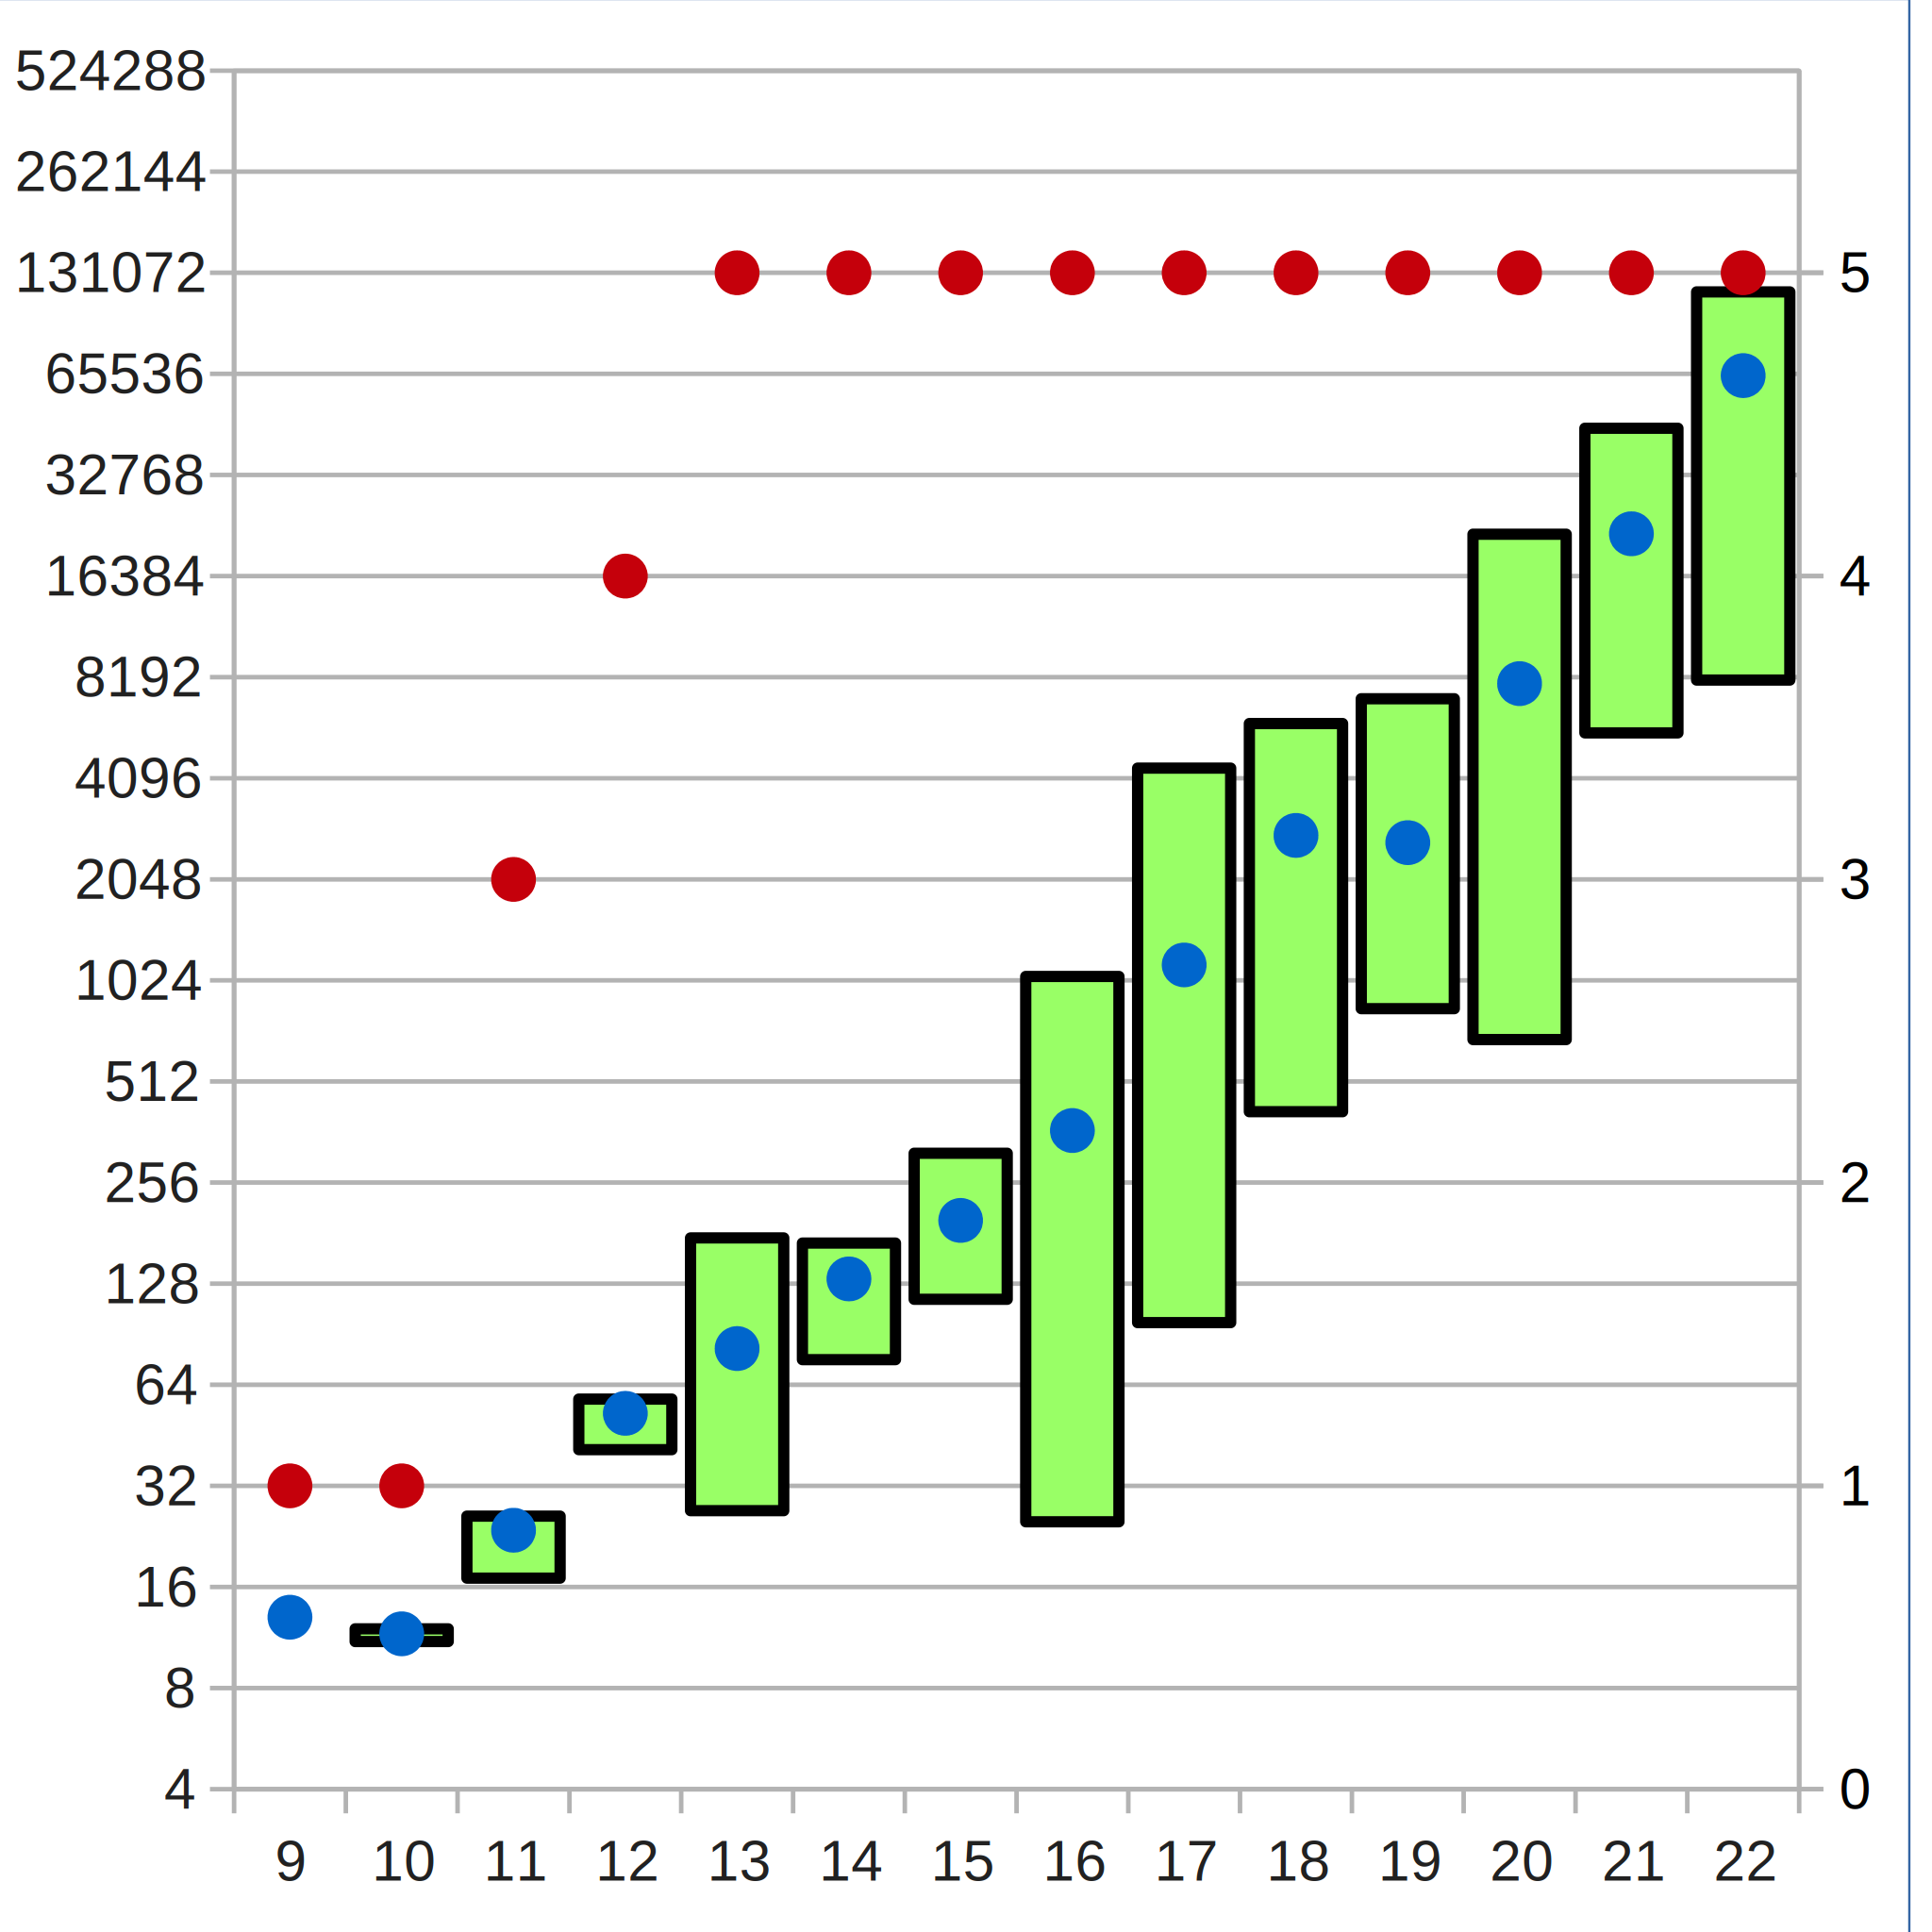
\includegraphics[scale=0.55]{images/data_dist_xor}
  \end{minipage}
  \caption{Ergebnisse mit Distanzklauseln}
  \label{fig:data_dist}
\end{figure}
\section{Test mit zusätzlichen Addiererklauseln} % 211 - 291
\label{sec:test_234}

Im Test aus Abschnitt \ref{sec:test_modul} wurden die modulspezifischen Klauseln getestet, jedoch zusätzliche Klauseln für den Addierer weggelassen.
Das betrifft die Klauseln aus Tabelle \ref{fig:additional_clauses_add}, die in diesem Test separat getestet werden.
Die Ergebnisse sind in Abbildung \ref{fig:data_add} dargestellt. Die Testlaufzeit beider Varianten sind mehr als doppelt so hoch und bei der
Anzahl der unterschiedlichen Lösungen lässt sich keine Veränderung erkennen.
\begin{figure}[!h]
  \centering
  \begin{minipage}[c]{0.45\textwidth}
  \begin{flushleft}Gesamtdauer ohne XOR: 410:59:52\end{flushleft}
  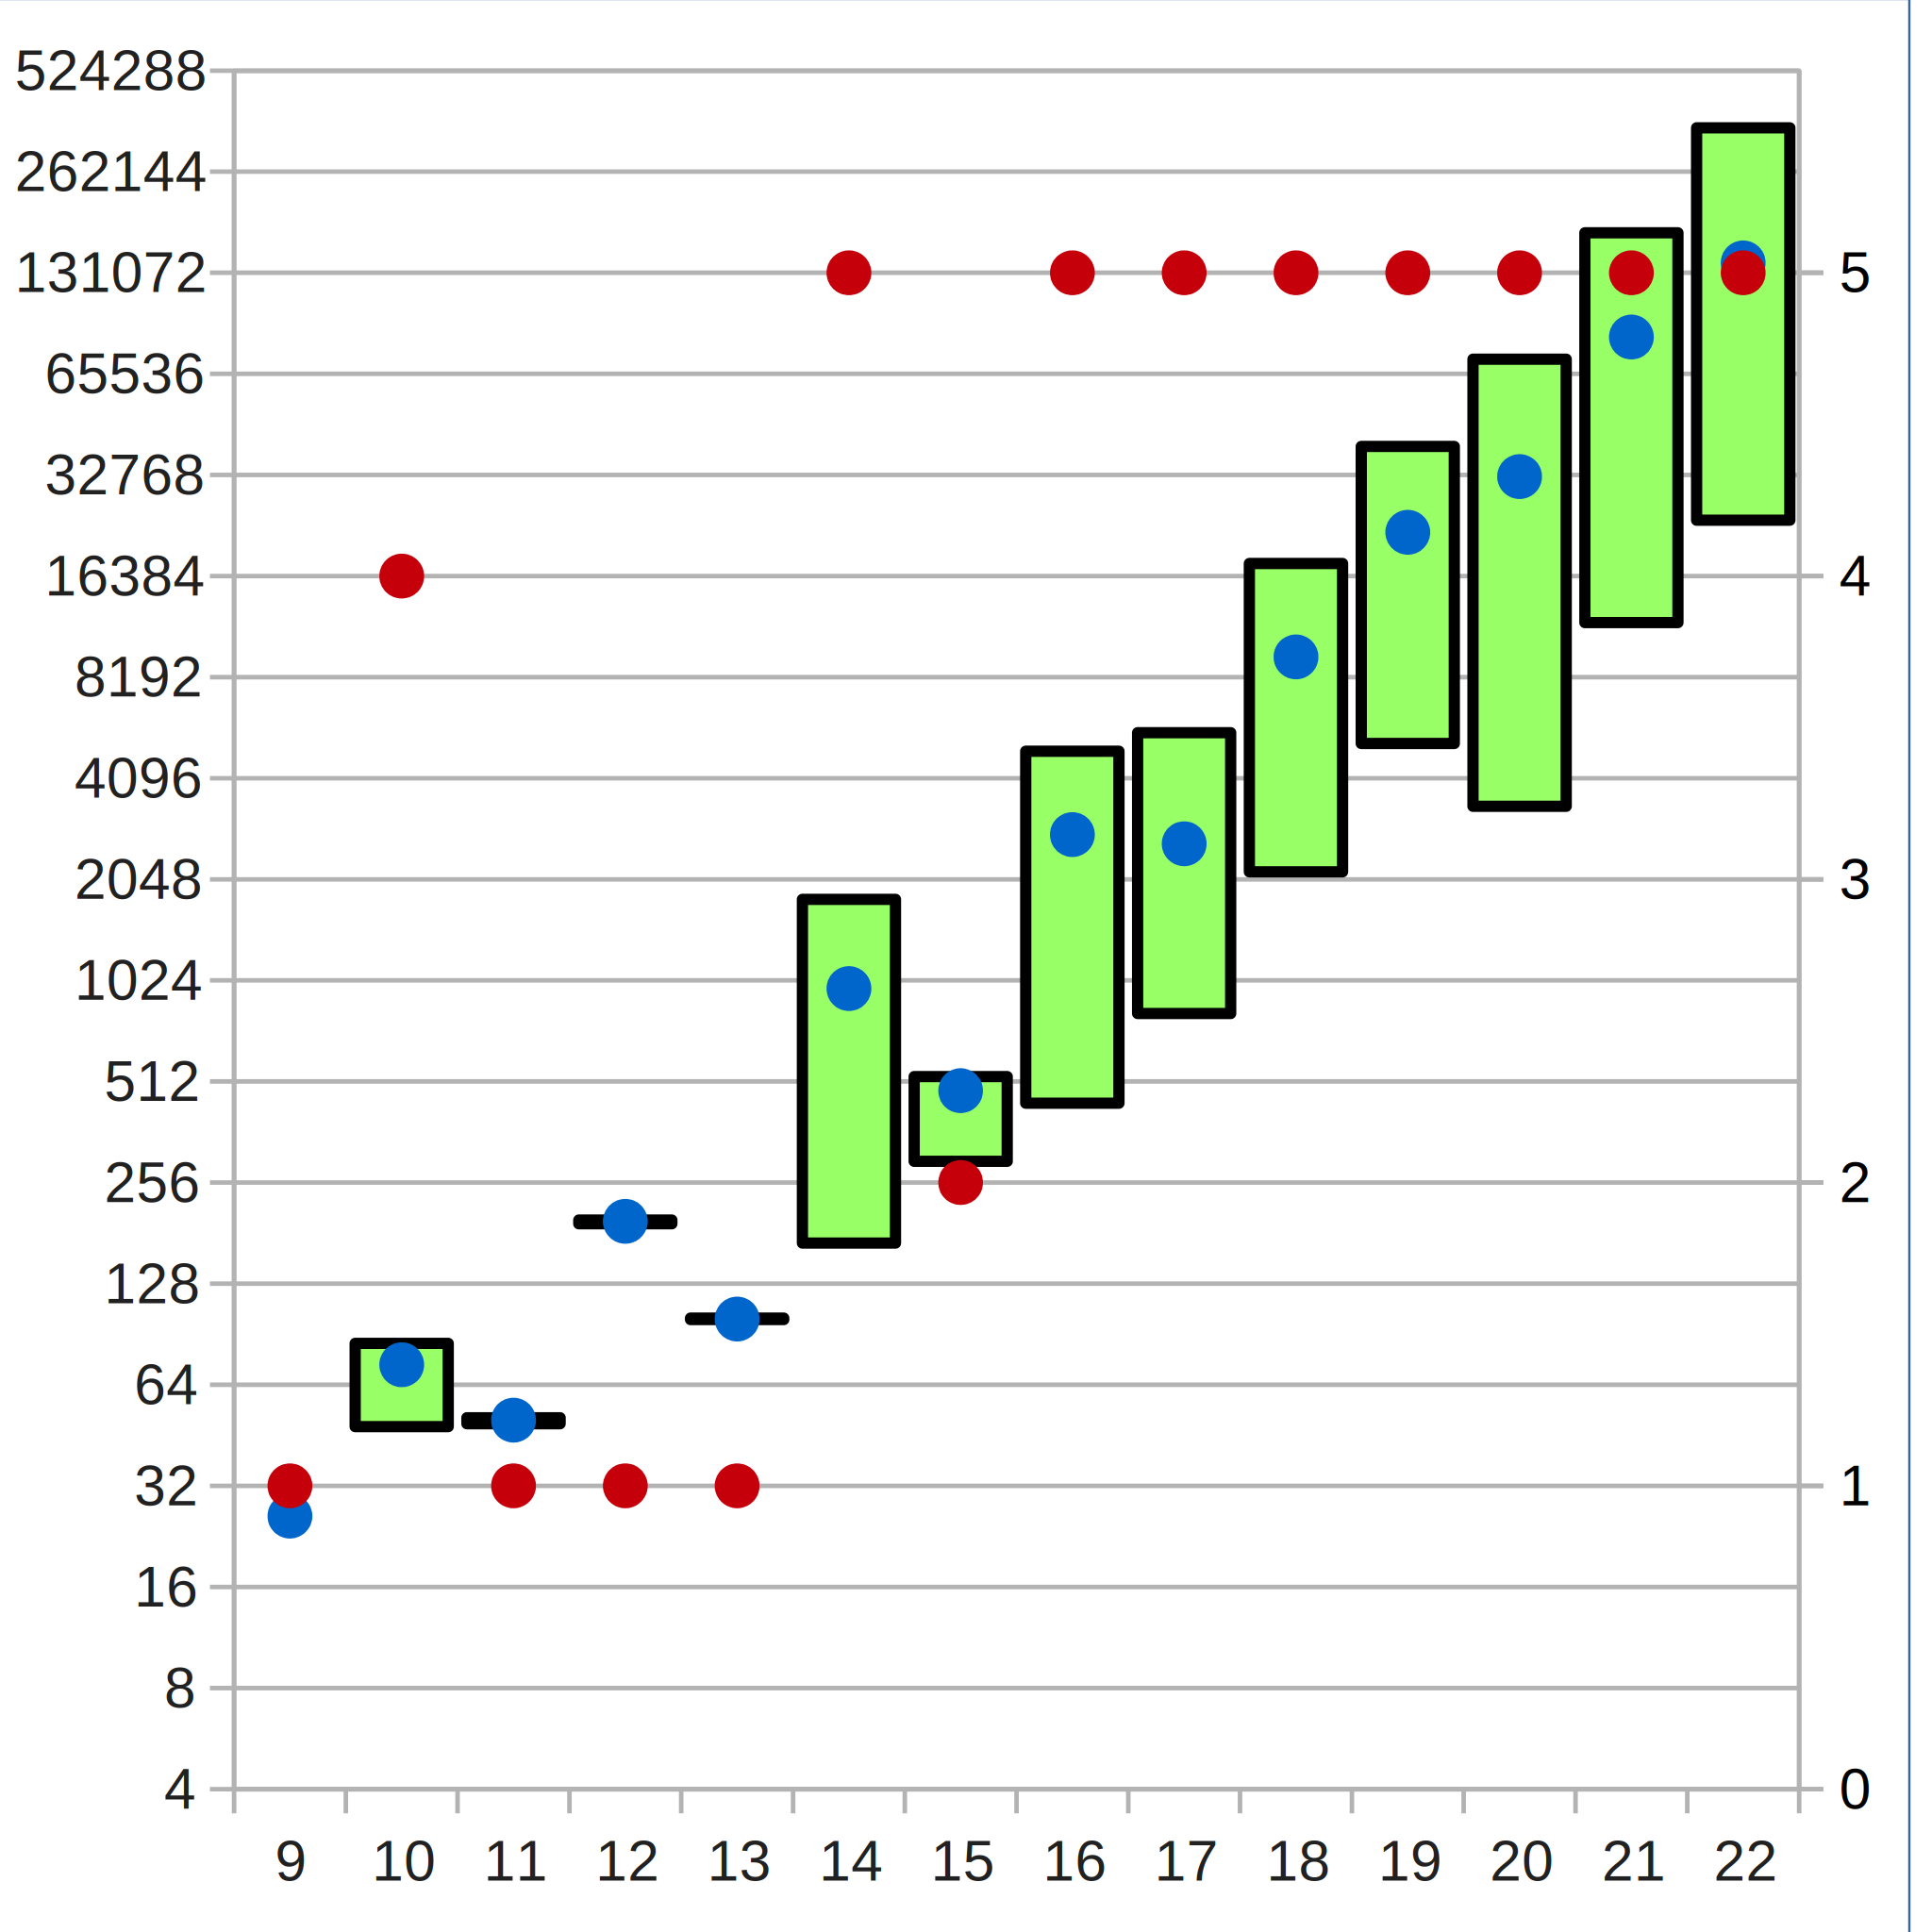
\includegraphics[scale=0.55]{images/data_add_knf}
  \end{minipage}
  \begin{minipage}[c]{0.09\textwidth}
  ~~
  \end{minipage}
  \begin{minipage}[c]{0.45\textwidth}
  \begin{flushleft}Gesamtdauer mit XOR: 491:53:48\end{flushleft}
  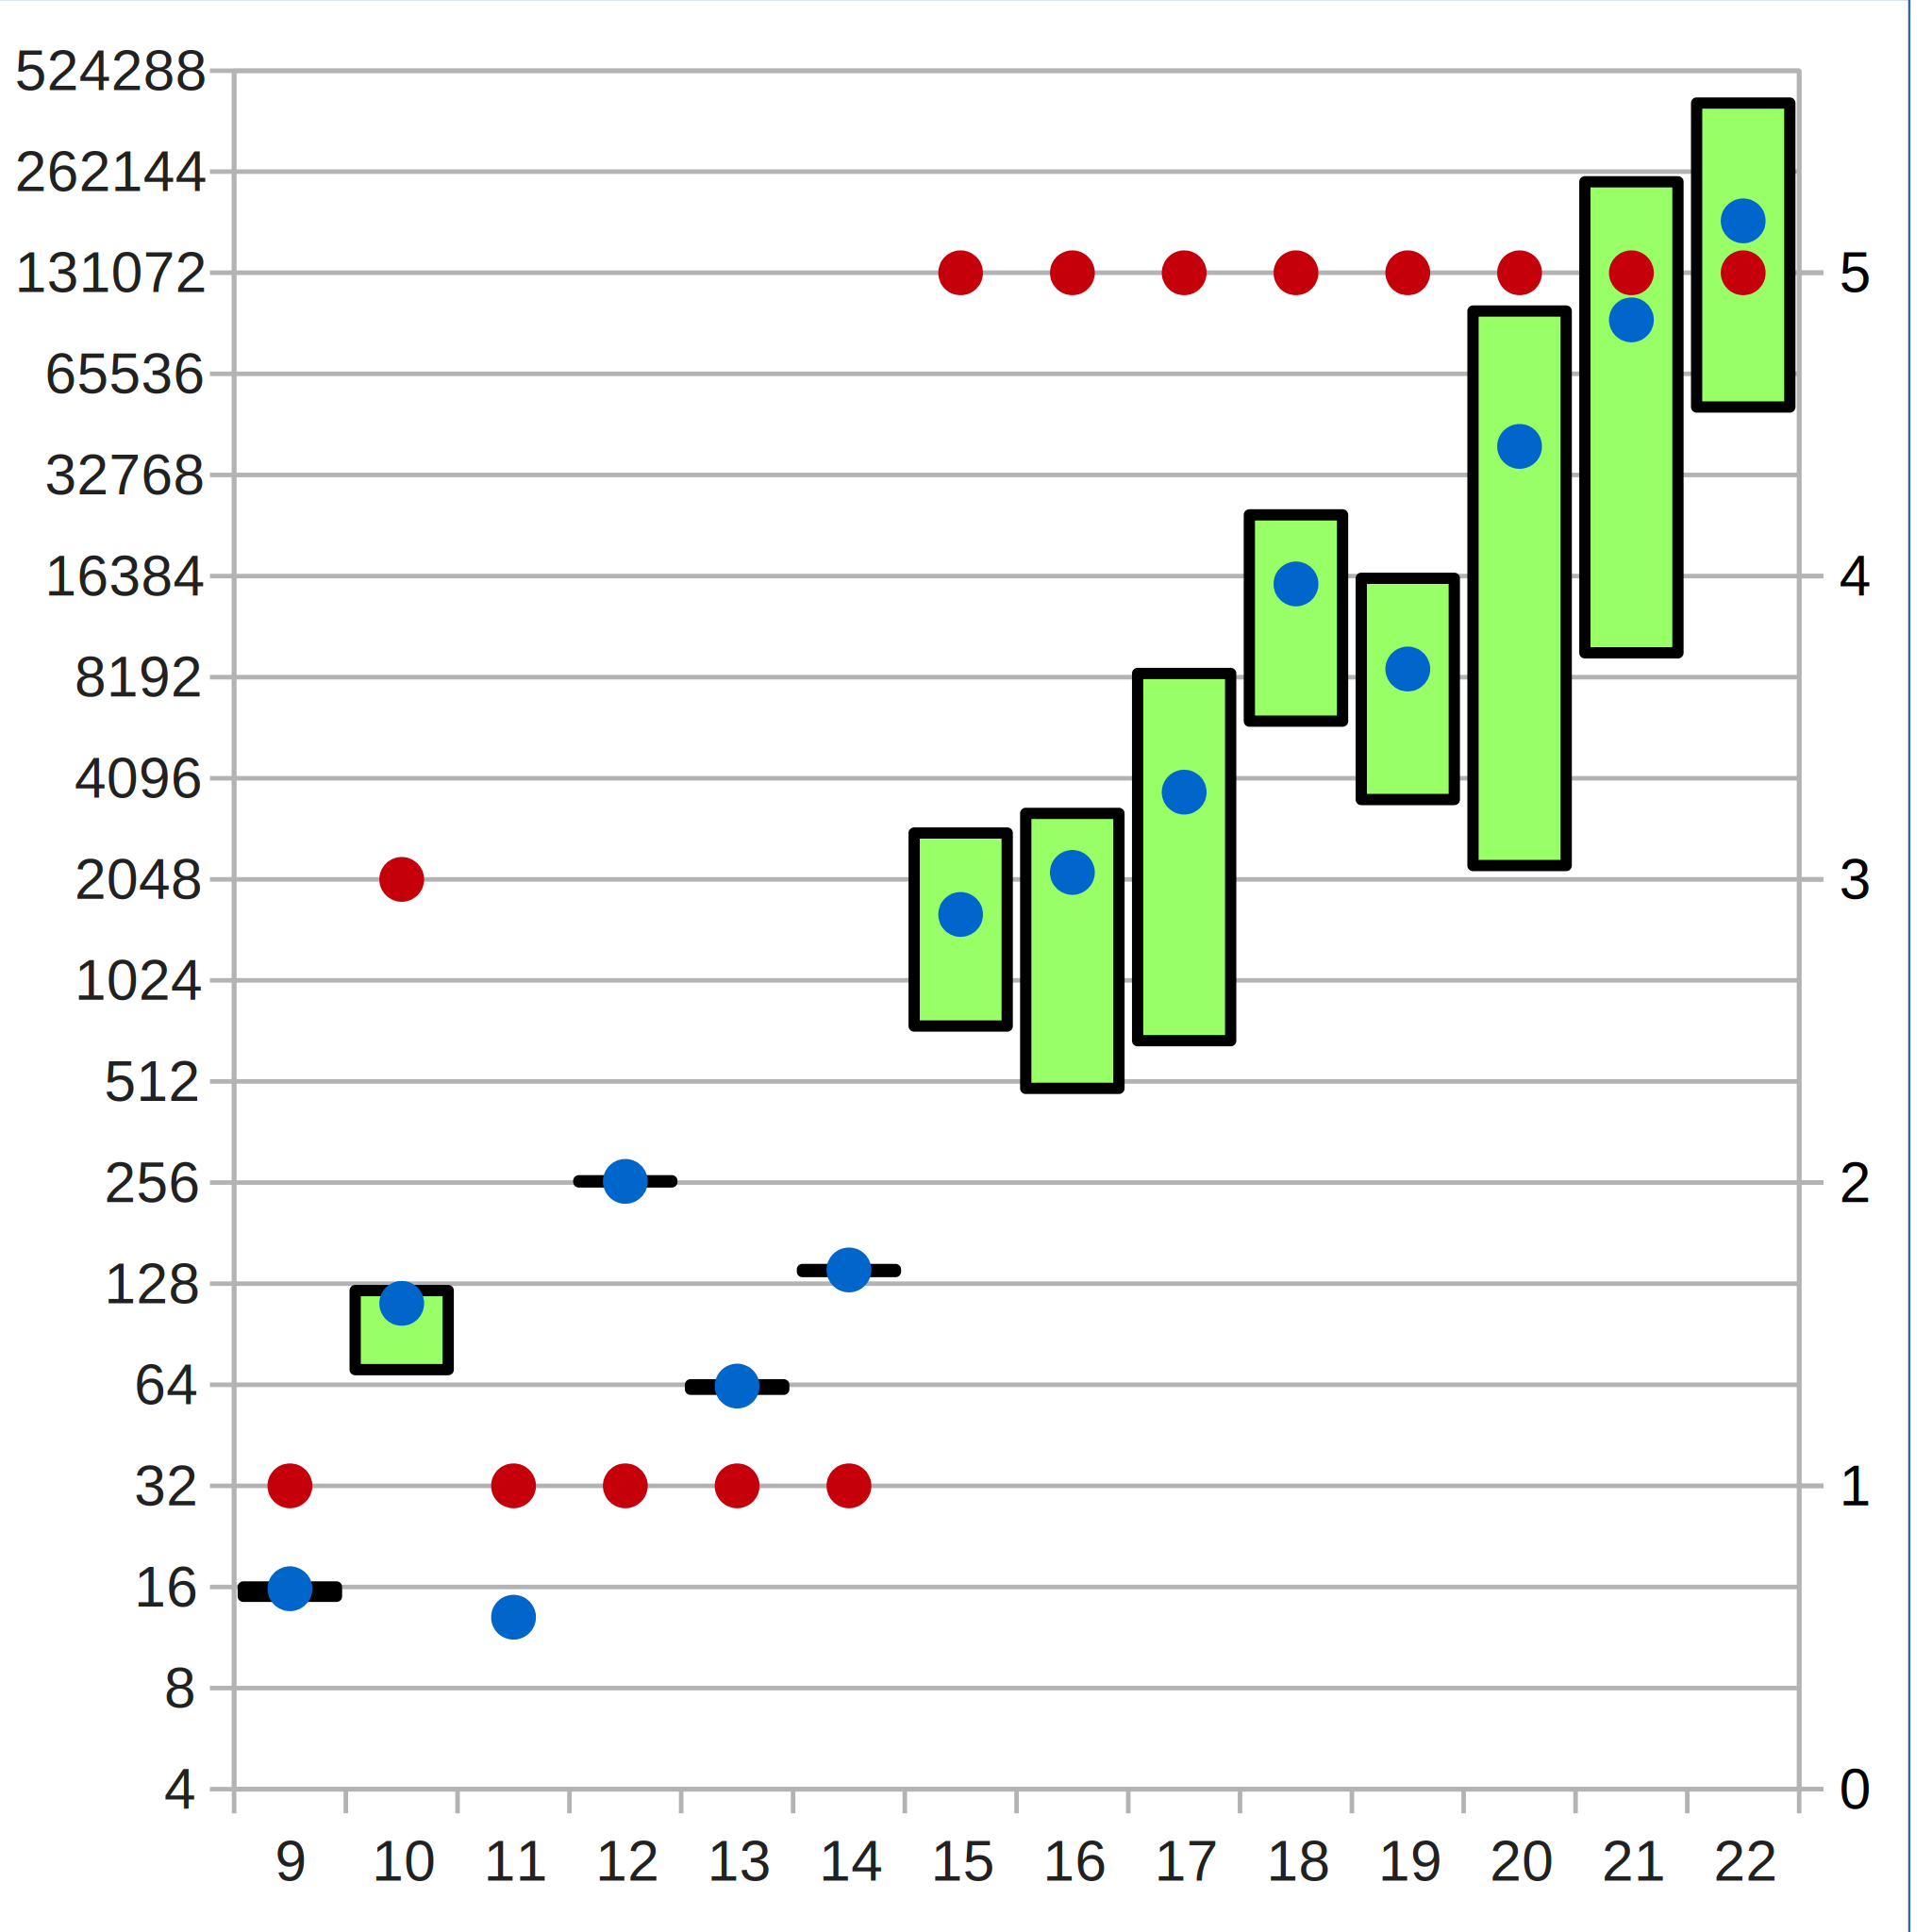
\includegraphics[scale=0.55]{images/data_add_xor}
  \end{minipage}
  \caption{Ergebnisse mit zusätzlichen Addiererklauseln}
  \label{fig:data_add}
\end{figure}
\section{Test mit zusätzlichem Wissen} % 106 - 59
\label{sec:test_knowledge}

In Abschnitt \ref{sec:ana:rundenfunktion} (Abbildung \ref{eq:calcD}) wurde zusätzliches Wissen über die Rundenfunktion ermittelt/beschrieben.
Für einen SAT-Solver mag dieses Wissen redundant sein und überflüssig erscheinen, da ein SAT-Solver nicht zwischen Vorwärts- und Rückwärts-Rechnen
unterscheidet. Jedoch werden durch dieses Wissen bestehende Module noch einmal anders verknüpft, was einem SAT-Solver die Möglichkeit bieten könnte,
einen alternativen Pfad zu nutzen und weitere Zusammenhänge zwischen Modulen zu erkennen. Nach dem selben Prinzip wäre es auch möglich, die Addition
von mehreren Summanden in unterschiedlicher Reihenfolge zusätzlich einzufügen. Der Fokus liegt jedoch darauf, nur festzustellen ob sich das
zusätzliche Wissen überhaupt auswirkt, weshalb auf die zusätzlichen Addierer verzichtet wird.

Ein Unterschied zu den vorhergehenden Tests ist, dass bei diesem Test nicht nur zusätzliche Klauseln notwendig sind sondern auch weitere Literale
benötigt werden. Außerdem wird ein zusätzliches Modul für die Subtraktion genutzt, welches bisher nicht näher beschrieben wurde, da es nach dem selben
Prinzip wie ein Addierer aufgebaut ist.

Die Ergebnisse sind in Abbildung \ref{fig:data_know} dargestellt. Während sich bei den vorhergehenden Tests die Laufzeit generell verkürzt oder
verlängert hat, verhalten sich die beiden Varianten in diesem Tests entgegengesetzt. Während sich die Laufzeit bei der Variante ohne XOR-Klauseln
leicht verlängert hat, hat sie sich bei der Variante mit XOR-Klauseln um 40\% verkürzt. Bei beiden Varianten ist jedoch ersichtlich, dass sich die
Anzahl der unterschiedlichen Lösungen speziell im Bereich mit wenig vorgegeben Bits erhöht hat. Das deutet darauf hin, dass CryptoMiniSat wieder
mehr rät. Bei der Variante mit XOR-Klauseln hat das jedoch gut geklappt. Fraglich ist aber, ob das dem Zufall geschuldet ist.
\begin{figure}[!h]
  \centering
  \begin{minipage}[c]{0.45\textwidth}
  \begin{flushleft}Gesamtdauer ohne XOR: 205:09:48\end{flushleft}
  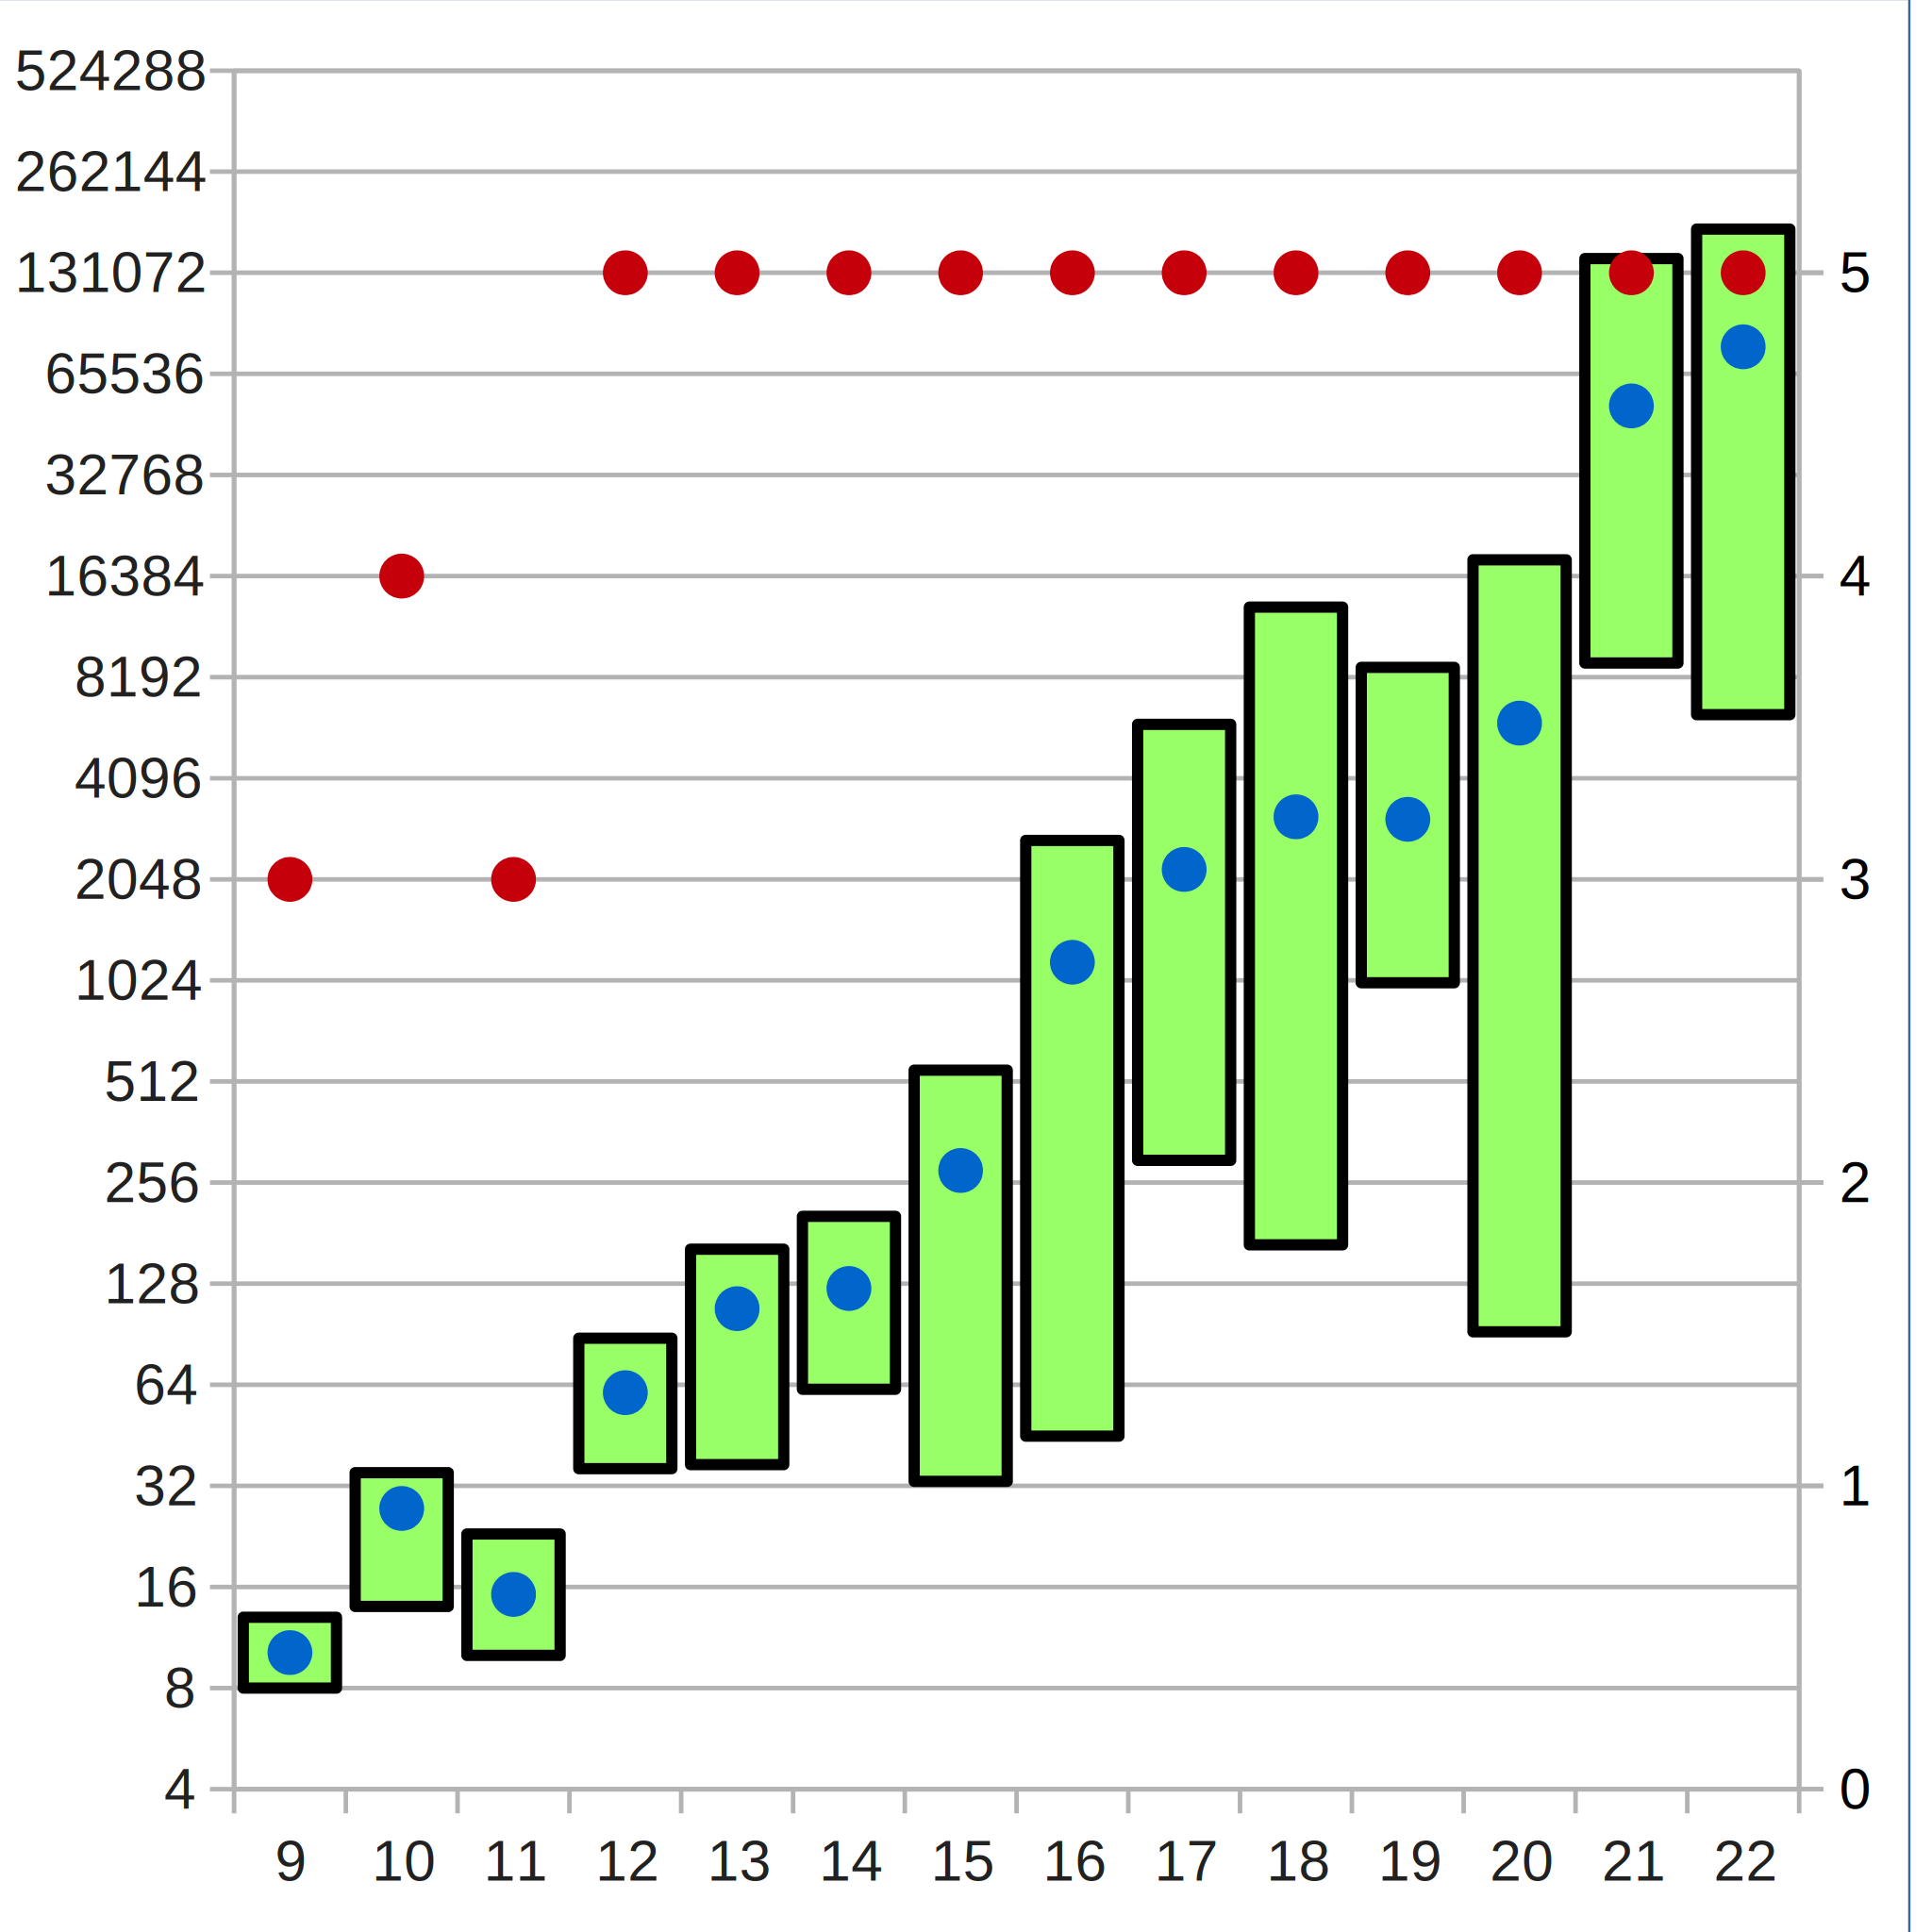
\includegraphics[scale=0.55]{images/data_know_knf}
  \end{minipage}
  \begin{minipage}[c]{0.09\textwidth}
  ~~
  \end{minipage}
  \begin{minipage}[c]{0.45\textwidth}
  \begin{flushleft}Gesamtdauer mit XOR: 100:41:09\end{flushleft}
  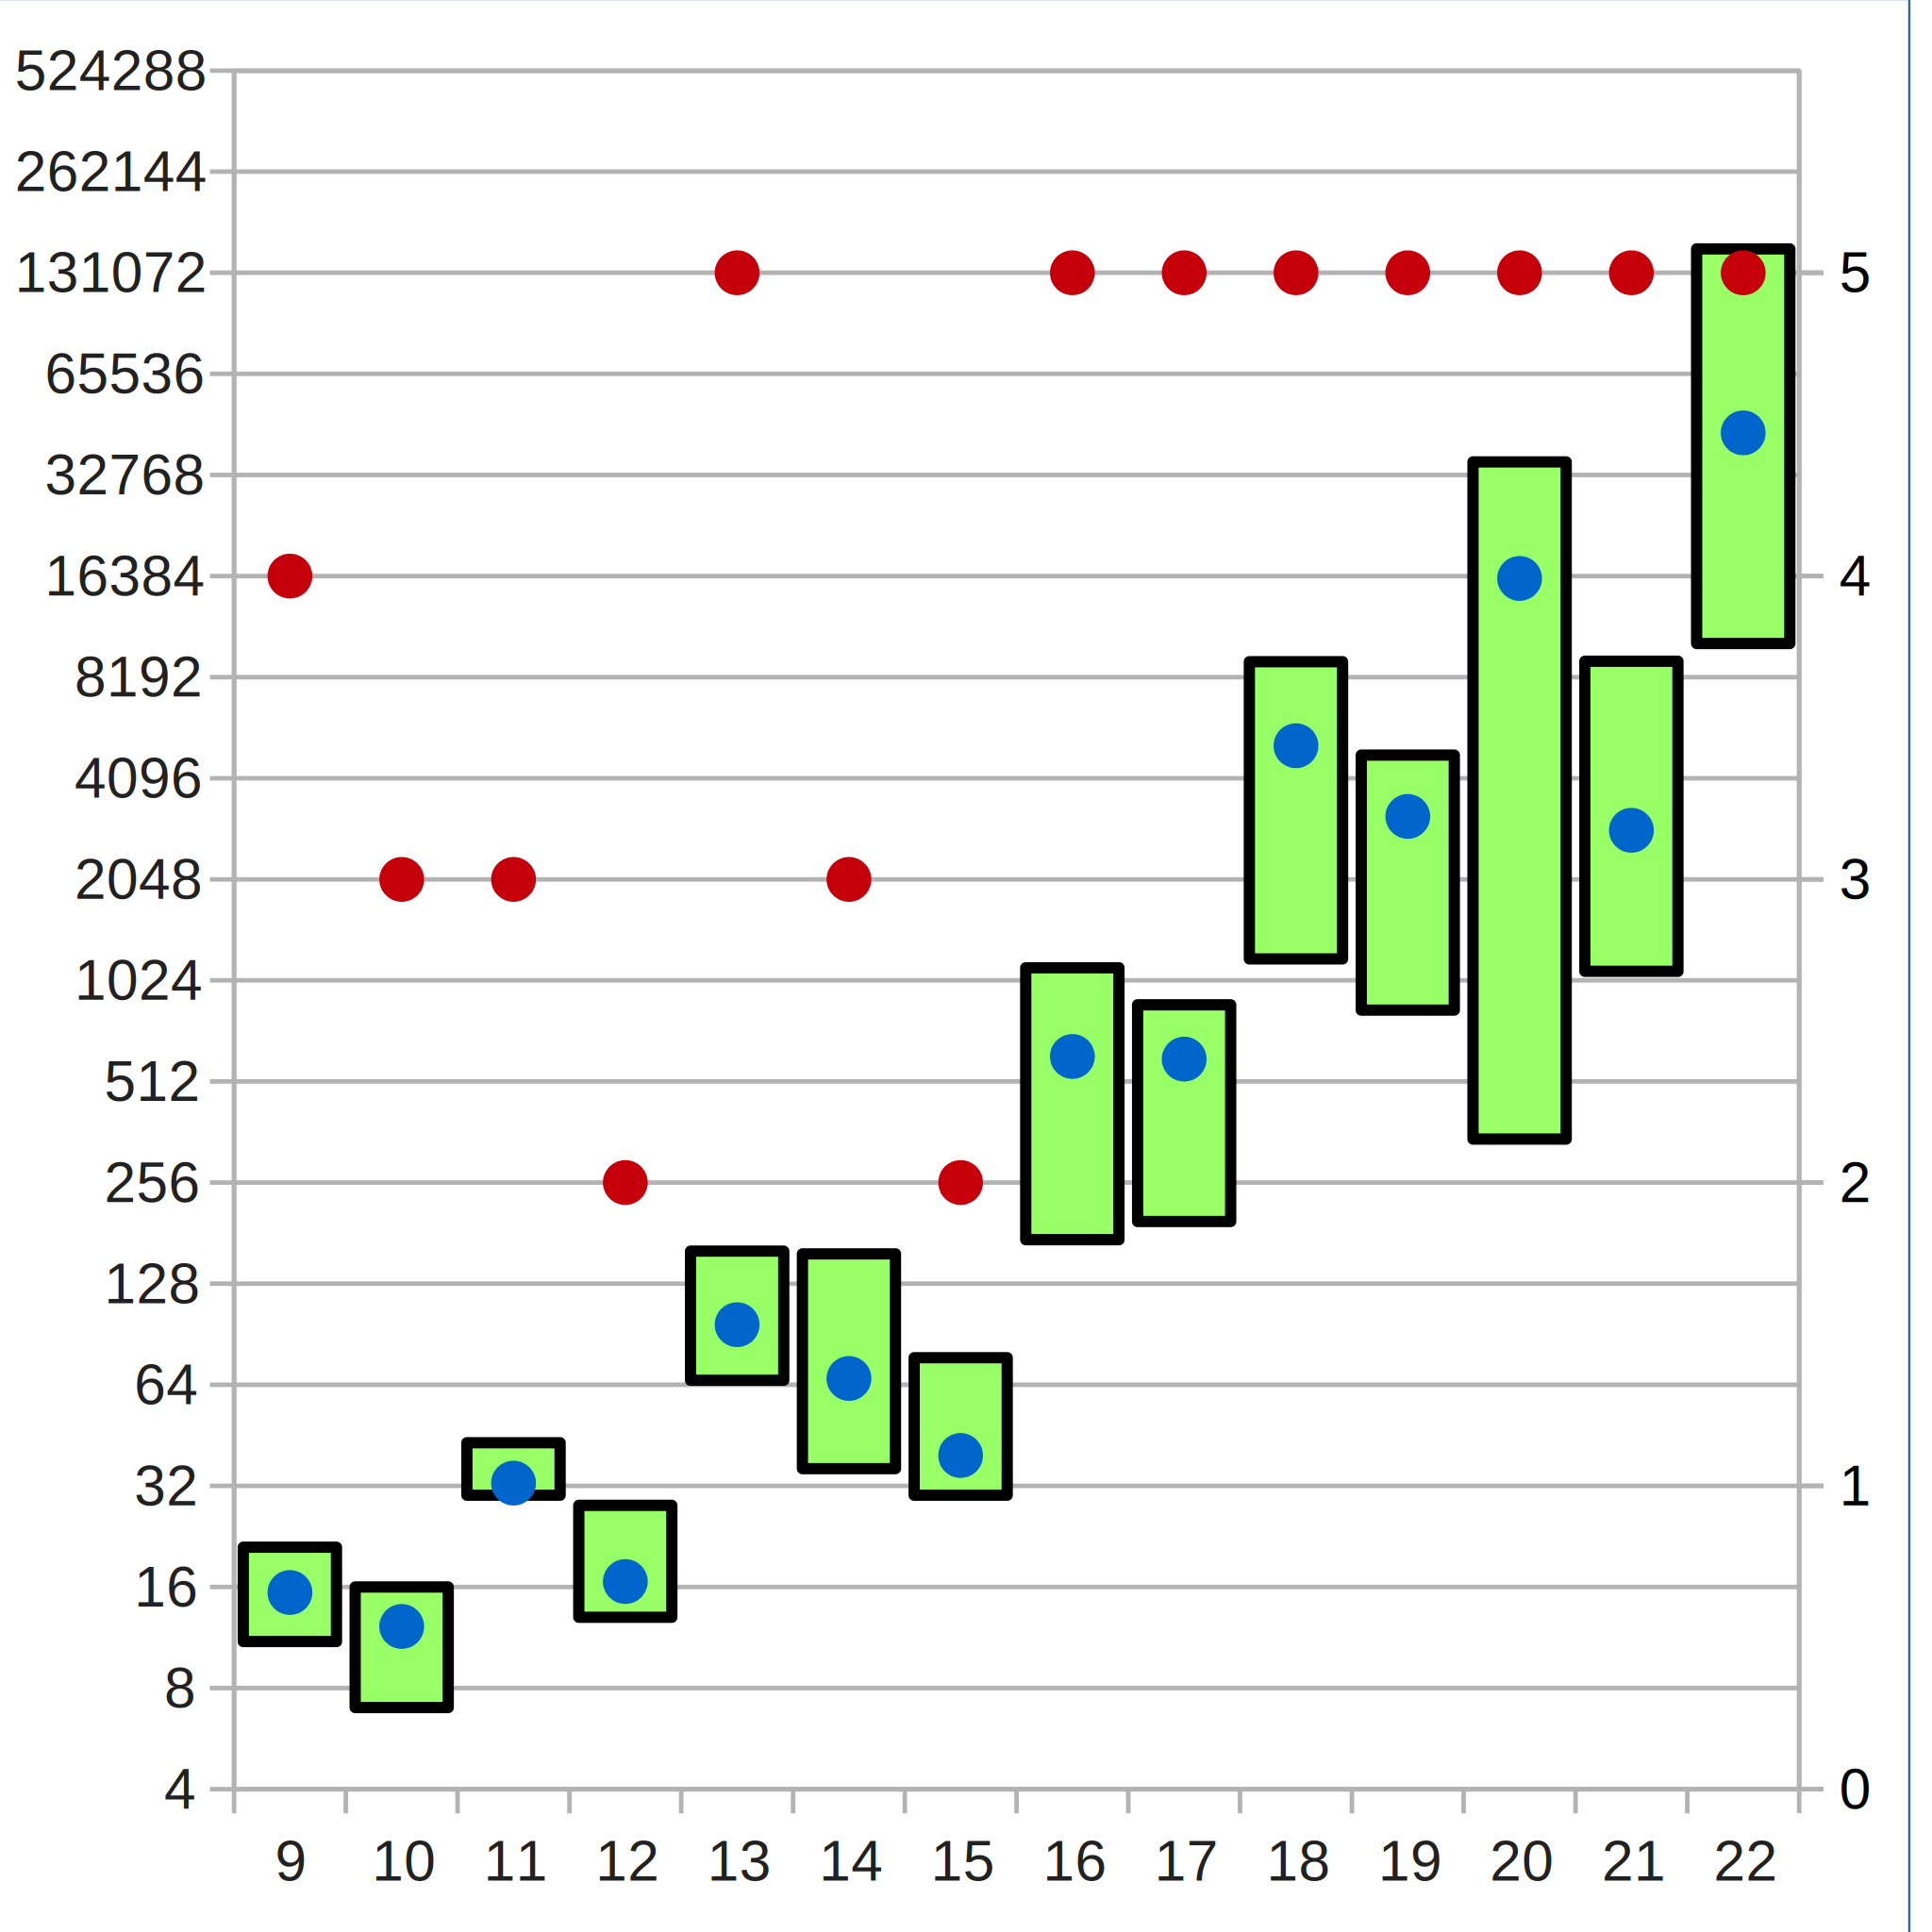
\includegraphics[scale=0.55]{images/data_know_xor}
  \end{minipage}
  \caption{Ergebnisse mit zusätzlichem Wissen}
  \label{fig:data_know}
\end{figure}
\section{Test mit allen vorteilhaften Klauseln} % 115 - 80
\label{sec:test_beste}

Die Ergebnisse sind in Abbildung \ref{fig:data_final} dargestellt.

\TODO{erledigen}

\begin{figure}[!h]
  \centering
  \begin{minipage}[c]{0.45\textwidth}
  \begin{flushleft}Gesamtdauer ohne XOR: 224:36:00\end{flushleft}
  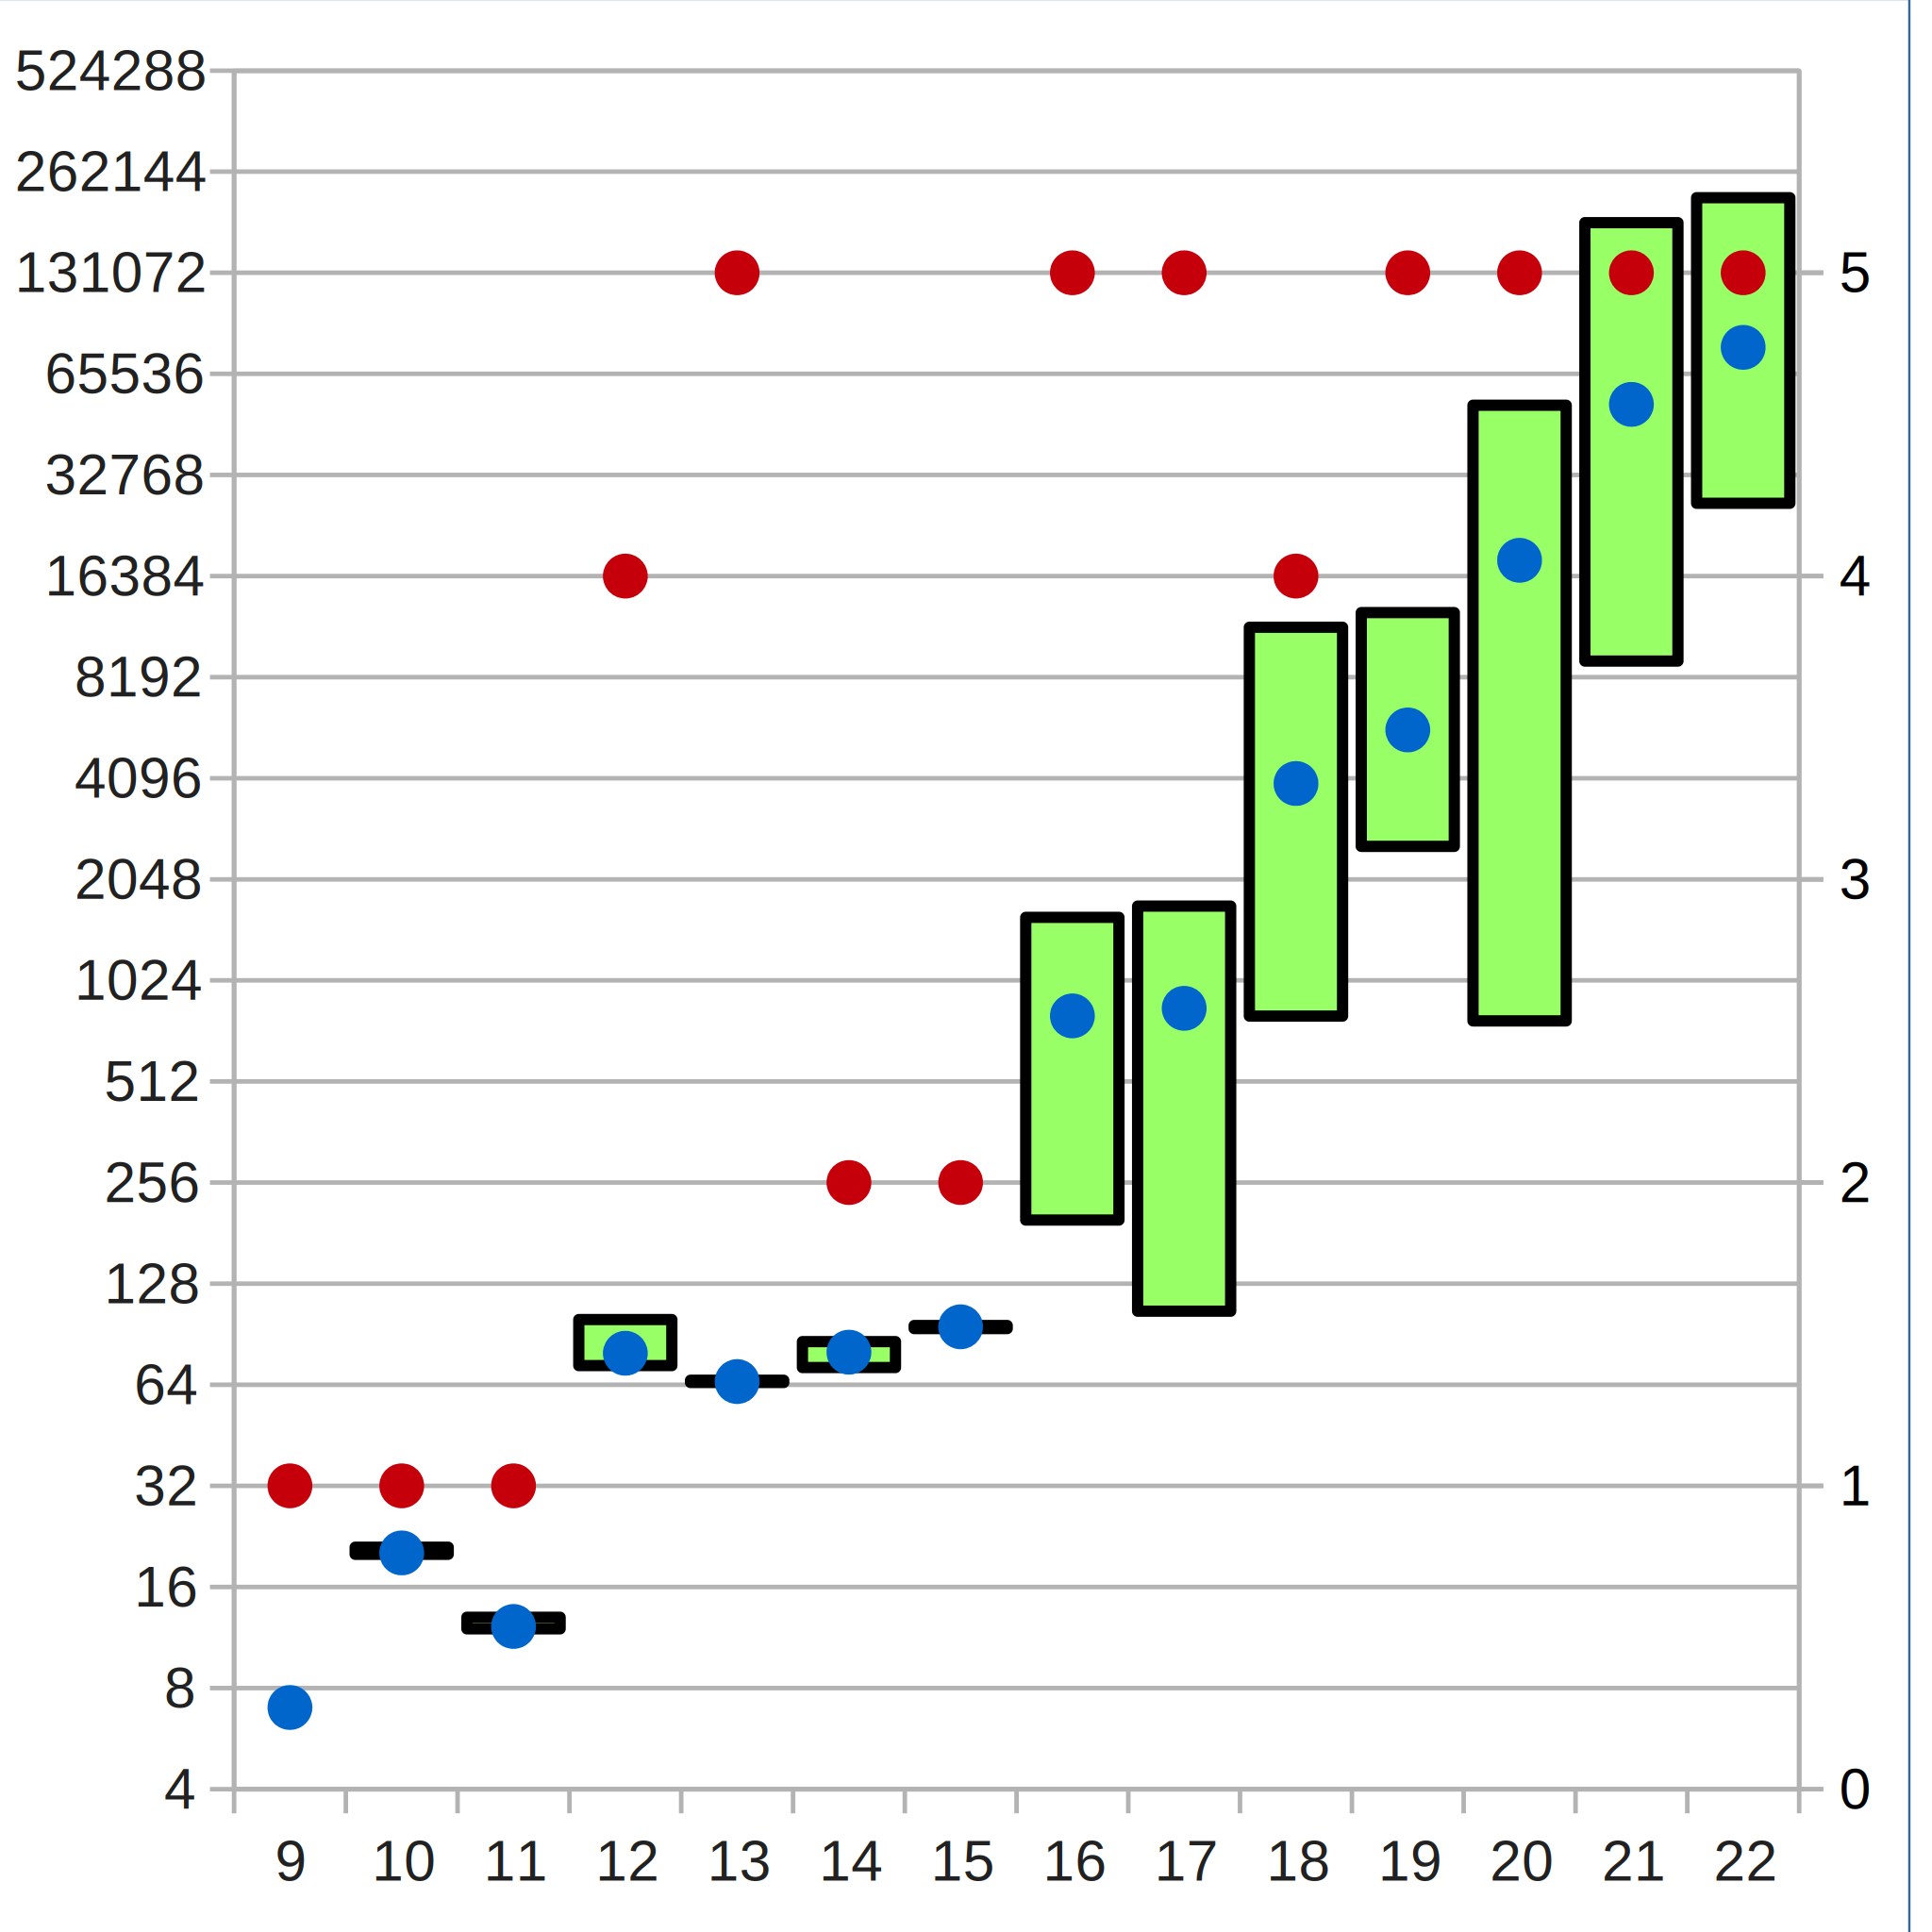
\includegraphics[scale=0.55]{images/data_final_knf}
  \end{minipage}
  \begin{minipage}[c]{0.09\textwidth}
  ~~
  \end{minipage}
  \begin{minipage}[c]{0.45\textwidth}
  \begin{flushleft}Gesamtdauer mit XOR: 136:37:46\end{flushleft}
  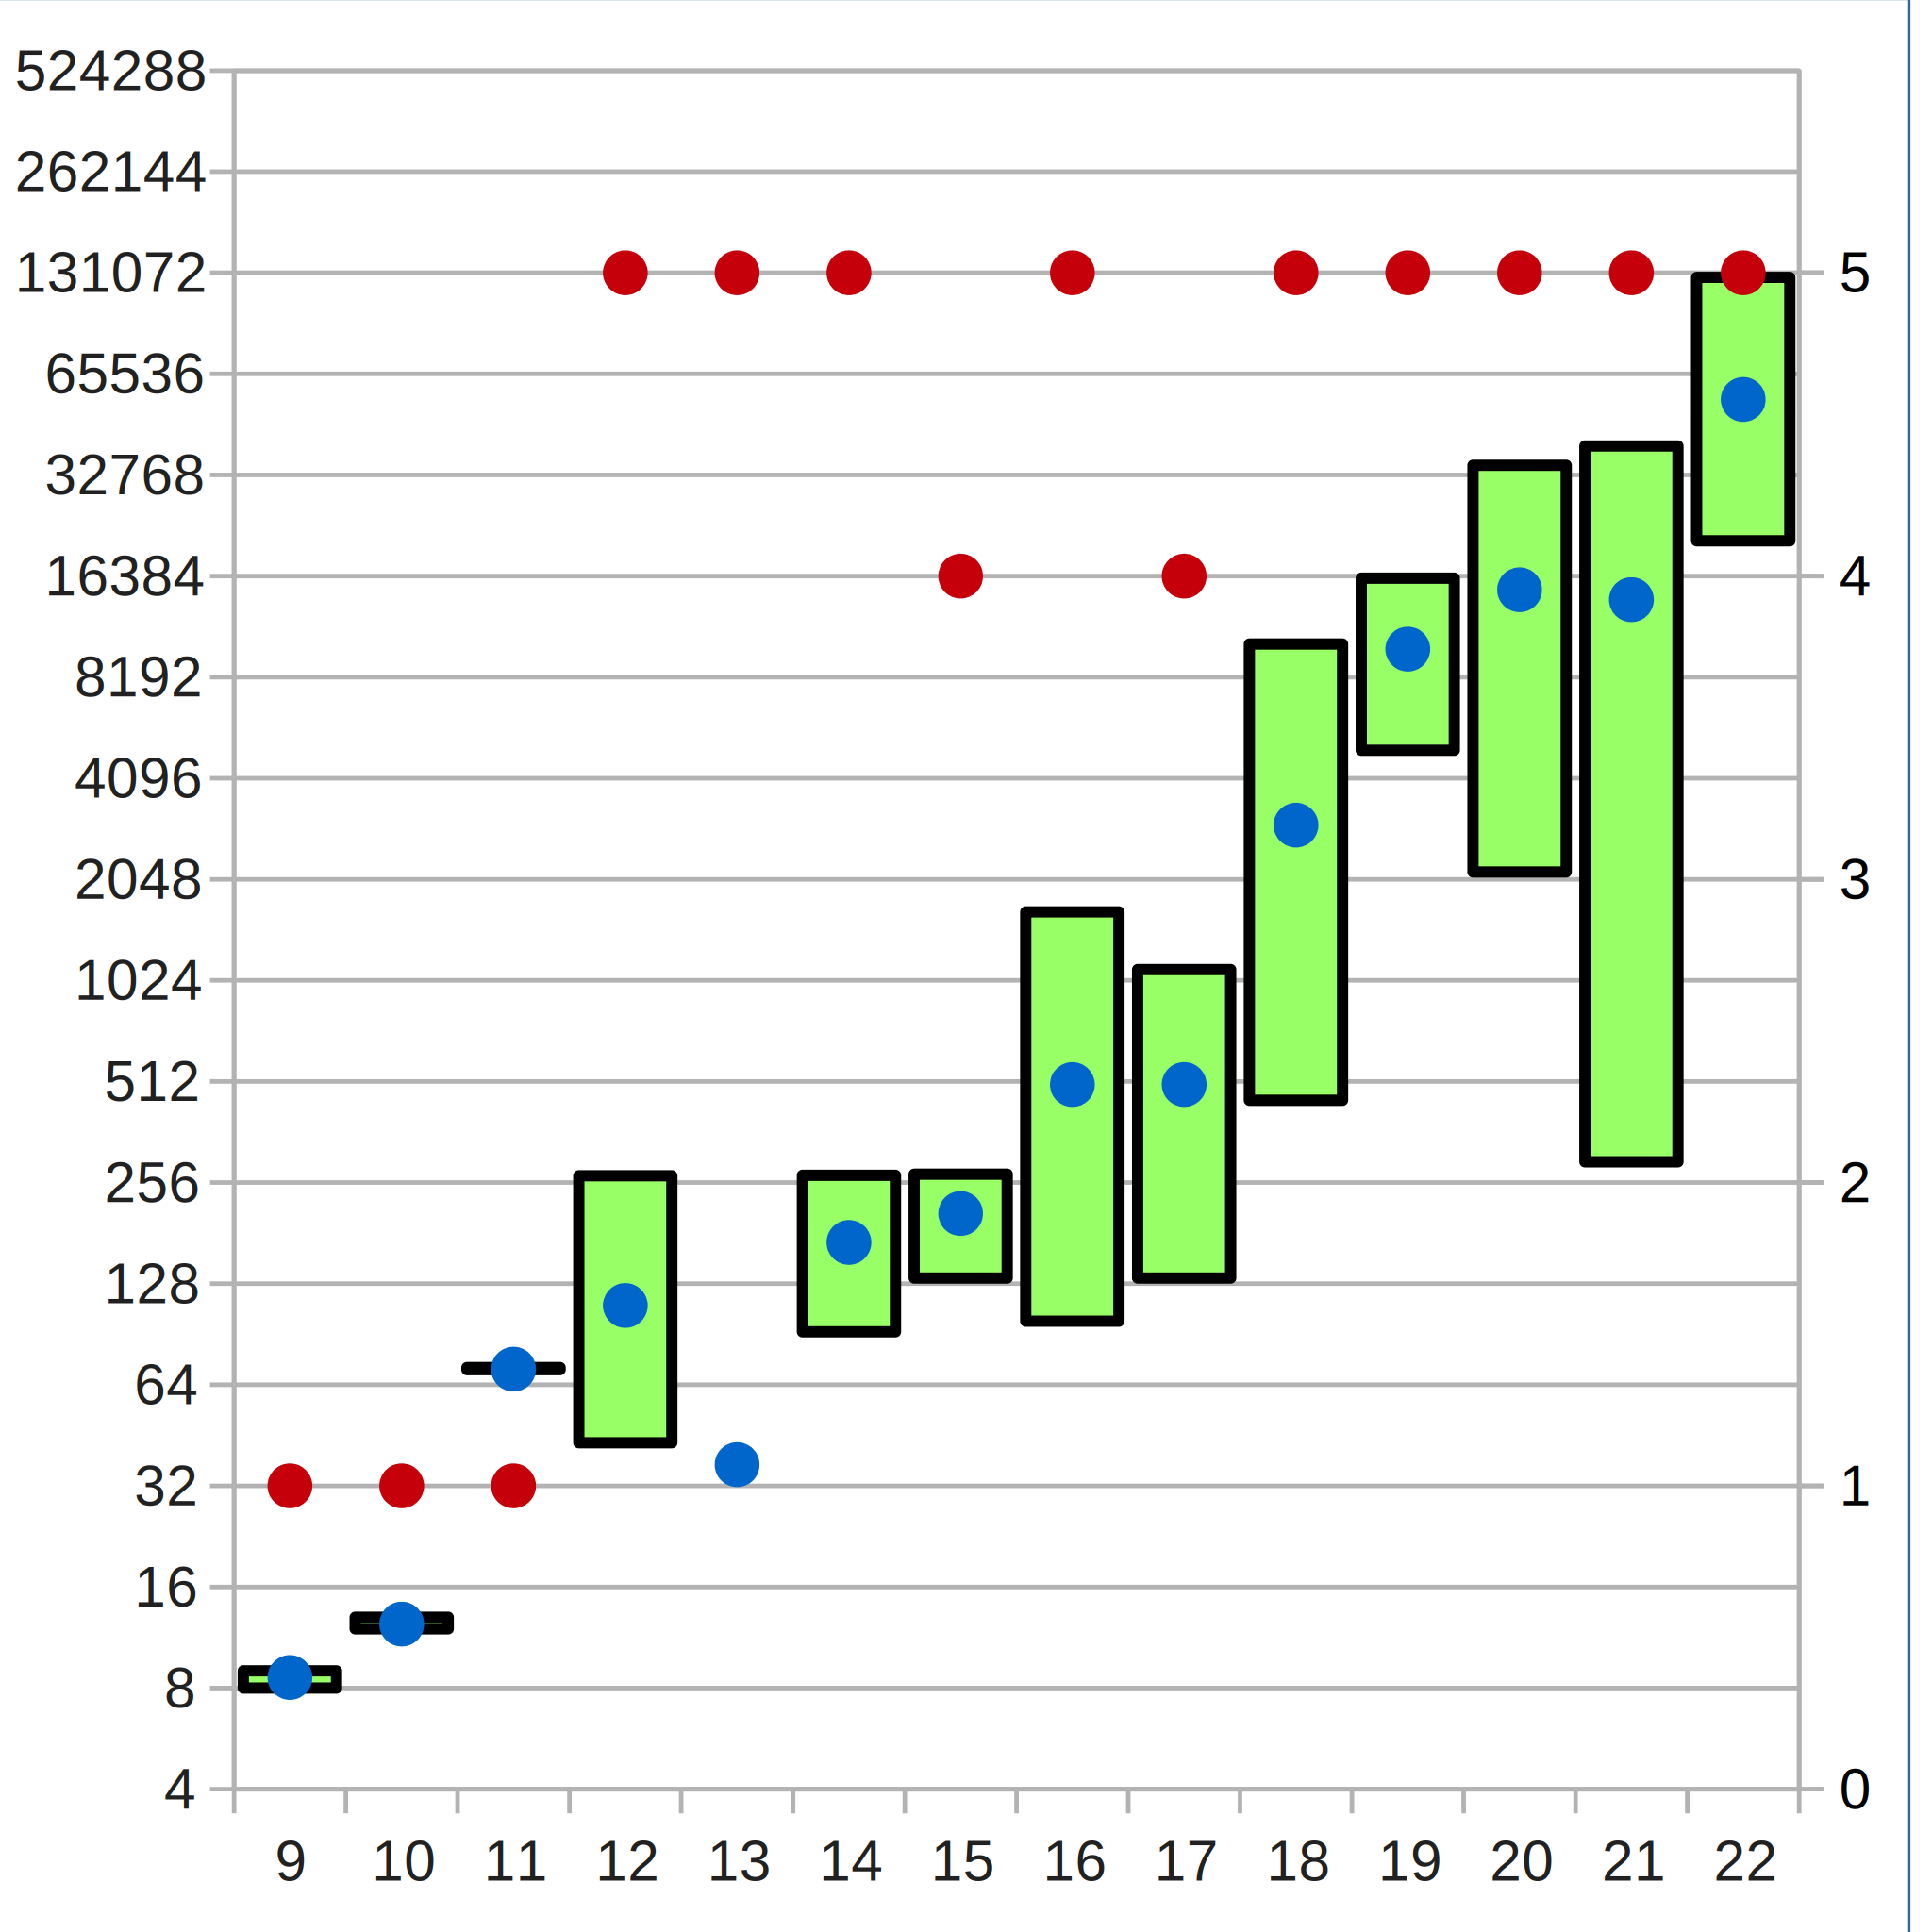
\includegraphics[scale=0.55]{images/data_final_xor}
  \end{minipage}
  \caption{Ergebnisse mit allen vorteilhaften Klauseln}
  \label{fig:data_final}
\end{figure}
\section{Vergleich der Resultate}

In allen Tests hat die XOR-Variante besser abgeschnitten als die Variante ohne XOR-Klauseln. Im Folgenden wird deshalb nur noch die XOR-Variante betrachtet.
Das beste Ergebnis haben die modulspezifischen Klauseln mit einer Reduktion der Testlaufzeit um fast 60\% erzielt. Auch die Distanzklauseln und das zusätzliche
Wissen haben die Testlaufzeit um 20\% bzw. 40\% reduziert. Negativ haben sich nur die zusätzlichen Addiererklauseln ausgewirkt. Die Vereinigung der positiv
getestet Klauseln hat nur eine Reduktion der Testlaufzeit um 20\% ergeben und konnte damit nicht an die 60\% der modulspezifischen Klauseln anknüpfen. Das ist
deshalb ein Problem, weil die modulspezifischen Klauseln mehr oder weniger "`abgeschlossen"' sind. Selbst wenn es in dieser Arbeit nicht gelungen ist, die
optimale "`vollständige"' Klauselmenge für die Module zu finden, ist diese doch begrenzt. Anders ist dies insbesondere bei den Distanzklauseln, da bei diesen
noch die Möglichkeit besteht viele weitere Klauseln zu ermitteln. Aus diesem Grund wird die Klauselmenge aus Abschnitt \ref{sec:test_beste} für die Evaluation
in Kapitel \ref{chp:evaluation} herangezogen. Gelingt es dieser Klauselmenge gegen andere Implementierungen zu bestehen, ist eine weitere Suche nach
Distanzklauseln möglicherweise sinnvoll.
